%Dies ist die Hauptseite des Dokumentes. Es werden u. a. alle Kapitel,
%Einstellung im Header eingebunden.  Veränderungen müssen in folgenden Dateien
%vorgenommen werden:
      %- config.tex
      %- Versionsübersicht
      %- einzelne Kapitel (evtl. erweitern)

%Hier sind alle Einstellungen enthalten, die sich auf das Seiten- und
%Dokumentenlayout beziehen

\documentclass[
  11pt,                   % Schriftgröße
  DIV12,
  german,                 % für Umlaute, Silbentrennung etc.
  oneside,                % einseitiges Dokument
  titlepage,              % es wird eine Titelseite verwendet
  parskip=half,           % Abstand zwischen Absätzen (halbe Zeile)
  headings=normal,        % Größe der Überschriften verkleinern
  captions=tableheading,  % Beschriftung von Tabellen unterhalb ausgeben
  final                   % Status des Dokuments (final/draft)
]{scrreprt}               %


%------Ändern von Schriftschnitten - (Muss ganz am Anfang stehen !) ------------
\usepackage{fix-cm}


%------Umlaute -----------------------------------------------------------------
%   Umlaute/Sonderzeichen wie äüöß können direkt im Quelltext verwenden werden.
%    Erlaubt automatische Trennung von Worten mit Umlauten.
\usepackage[T1]{fontenc}
\usepackage[utf8]{inputenc}

%------Anpassung der Landessprache----------------------------------------------
\usepackage[ngerman]{babel}

%------Einfache Definition der Zeilenabstände und Seitenränder------------------
\usepackage{geometry}
\usepackage{setspace}

%------Schriftgrößenanpassung von einzelnen Textpassagen------------------------
\usepackage{relsize}

%------Trennlinien in Kopf- und Fusszeile
\usepackage[headsepline, footsepline, ilines]{scrpage2}

%------Grafiken und Farben -----------------------------------------------------
\usepackage{xcolor}
\usepackage{graphicx}

%------Packet zum Sperren, Unterstreichen und Hervorheben von Texten------------
\usepackage{soul}

%------ergänzende Schriftart----------------------------------------------------
\usepackage{helvet}

%------Lange Tabellen-----------------------------------------------------------
\usepackage{longtable}
\usepackage{array}
\usepackage{ragged2e}
\usepackage{lscape}

%------PDF-Optionen-------------------------------------------------------------
\usepackage[
  bookmarks,
  bookmarksopen=true,
  colorlinks=true,
  linkcolor=black,        % einfache interne Verknüpfungen
  anchorcolor=black,      % Ankertext
  citecolor=black,        % Verweise auf Literaturverzeichniseinträge im Text
  filecolor=black,        % Verknüpfungen, die lokale Dateien öffnen
  menucolor=black,        % Acrobat-Menüpunkte
  urlcolor=black,         % Farbe für URL-Links
  backref,                % Zurücktext nach jedem Bibliografie-Eintrag als
                          % Liste von Überschriftsnummern
  pagebackref,            % Zurücktext nach jedem Bibliografie-Eintrag als
                          % Liste von Seitenzahlen
  plainpages=false,       % zur korrekten Erstellung der Bookmarks
  pdfpagelabels,          % zur korrekten Erstellung der Bookmarks
  hypertexnames=false,    % zur korrekten Erstellung der Bookmarks
  linktocpage             % Seitenzahlen anstatt Text im Inhaltsverzeichnis verlinken
  ]{hyperref}






      % enthält eingebundene Packete

%------Seitenränder-------------------------------------------------------------
\geometry{verbose,                     % zeigt die eingestellten Parameter beim
                                       % Latexlauf an
      paper=a4paper,                   % Papierformat
      top=25mm,                        % Rand oben
      left=25mm,                       % Rand links
      right=25mm,                      % Rand rechts
      bottom=45mm,                     % Rand unten
      pdftex                           % schreibt das Papierformat in die
                                       % Ausgabe damit Ausgabeprogramm
                                       % Papiergröße erkennt
  }

%Seitenlayout
\onehalfspace        % 1,5-facher Abstand

%------Kopf- und Fußzeilen -----------------------------------------------------
\pagestyle{scrheadings}

%------Kopf- und Fußzeile auch auf Kapitelanfangsseiten ------------------------
\renewcommand*{\chapterpagestyle}{scrheadings}

%------Schriftform der Kopfzeile -----------------------------------------------
\renewcommand{\headfont}{\normalfont}

%----Spezielle Befehle
\newcommand{\lfk}[1]{$\langle LF#1\rangle$}

%----Farben
\definecolor{tubsRed}{cmyk}{0.1,1.0,0.8,0.0}
\definecolor{tuRed}{cmyk}{0.1,1.0,0.8,0.0}

%------Kopfzeile----------------------------------------------------------------
\setheadsepline{1pt}[\color{tuRed}]
\setlength{\headheight}{21mm}        % Höhe der Kopfzeile
\ihead{\large{\textsc{\praktikumTitel}}\\    % Text in der linken Box
       \small{\projektTitel}}
\chead{}                            % Text in der mittleren Box

%----Fusszeile
\setfootsepline{1pt}[\color{tuRed}]
\cfoot{}                            % Text in mittlerer Box
\ofoot{\pagemark}                    % Seitenzahl in rechter Box



%------Labels mit eigenem Text für \ref ----------------------------------------
\makeatletter
\def\namedlabel#1#2{\begingroup
#2%
\def\@currentlabel{#2}%
\phantomsection\label{#1}\endgroup
}
\makeatother


%------Neue Environments -------------------------------------------------------

\newcommand{\refsetcounter}[2]{\setcounter{#1}{#2}\addtocounter{#1}{-1}\refstepcounter{#1}}

%Funktion im Pflichtenheft
\newcounter{functioncount} 
\newenvironment{function}[2]{\refsetcounter{functioncount}{#1}\large\textbf{\sffamily{#2 }}\namedlabel{F#1}{$\langle F#1\rangle$}\normalsize\begin{description}\setlength{\itemsep}{-5pt}}{\end{description}}

%Daten im Pflichtenheft
\newcounter{datacount} 
\newenvironment{data}[2]{\refsetcounter{datacount}{#1}\textbf{#2} \namedlabel{D#1}{$\langle D#1\rangle$}\\}{}

%Kriterien im Pflichtenheft
\newcounter{mustcount} 
\newcommand{\must}[2]{\refsetcounter{mustcount}{#1}\namedlabel{RM#1}{$\langle RM#1\rangle$} #2\\}

\newcommand{\should}[2]{\refsetcounter{datacount}{#1}\namedlabel{RS#1}{$\langle RS#1\rangle$} #2\\}

\newcommand{\could}[2]{\refsetcounter{datacount}{#1}\namedlabel{RC#1}{$\langle RC#1\rangle$} #2\\}

\newcommand{\wont}[2]{\refsetcounter{datacount}{#1}\namedlabel{RW#1}{$\langle RW#1\rangle$} #2\\}

%Qualitätsanforderungen im Pflichtenheft
\newcommand{\qualityReq}[2]{\refsetcounter{datacount}{#1}\namedlabel{Q#1}{$\langle Q#1\rangle$} #2\\}

% Benutzeroberflächen im Pflichtenheft
\newcounter{uicount}
\newenvironment{ui}[2]{\refsetcounter{uicount}{#1}\textbf{#2} \namedlabel{UI#1}{$\langle UI#1\rangle$}\\}{}

% Klassen
\newcounter{classcount}
\newenvironment{class}[2]{\refsetcounter{classcount}{#1}\textbf{#2}\namedlabel{CL#1}{$\langle CL#1\rangle$}\begin{description}\setlength{\itemsep}{-5pt}}{\end{description}}

% Entitäten
\newcounter{entitycount}
\newenvironment{entity}[2]{\refsetcounter{entitycount}{#1}\textbf{#2} \namedlabel{E#1}{$\langle E#1\rangle$}\\}{}

% Component
\newcounter{componentcount}
\newenvironment{component}[2]{\refsetcounter{componentcount}{#1}\textbf{Komponente \namedlabel{C#1}{$\langle C#1\rangle$}: #2}\\}{}

% Interface
\newcounter{interfacecount}
\newenvironment{interface}[2]{\refsetcounter{interfacecount}{#1}\textbf{Schnittstelle \namedlabel{I#1}{$\langle I#1\rangle$}: #2}\\}{}

% Testfall
\newcounter{testcasecount}
\newenvironment{testcase}[2]{\clearpage\refsetcounter{testcasecount}{#1}\subsection{Testfall $\langle T#1\rangle$ - #2}\label{T#1}\begin{description}\setlength{\itemsep}{-5pt}}{\end{description}}
           % Diese Datei enthält alle
                                           % Layouteinstellungen
\newcommand{\dokumentTitel}{Pflichtenheft}
% Definition von globalen Parametern, die derzeit auf der Titelseite und in der
% Kopfzeile verwendet werden. Der in <> gesetzte Text ist zu verändern.

\newcommand{\praktikumTitel}{Das Gro\ss{}e SQL-Spiel}
\newcommand{\projektTitel}{The SQL-Alchemist}
\newcommand{\institut}{
	Institut f\"ur Informationssysteme\\
	Prof. Dr. Wolf-Tilo Balke\\
	M\"uhlenpfordtstra\ss{}e 23, 2.OG\\
	D-38106 Braunschweig\\
}
\newcommand{\institutsLogo}{common/ISF_Logo.pdf}
\newcommand{\betreuer}{Jan-Christoph Kalo}

%------Beginn des Gesamtdokumentes----------------------------------------------
\begin{document}

%------Eingebundene Seiten, Verzeichnisse bzw. Kapitel--------------------------
% Dies ist die Titelseite.
% Die Ausgabe darf 1 Seite nicht überschreiten, also ggf. Abstände anpassen
% Die Angabe in [...] gibt den Abstand nach der entsprechenden Zeile an.


%----Stil dieser Seite----------------------------------------------------------
\thispagestyle{plain}      % Kopfzeile bleibt leer

%----Beginn der Titelseite------------------------------------------------------
\begin{titlepage}

%----eingebundenes Logo der TU--------------------------------------------------
%\setlength{\unitlength}{1mm}
%  \begin{picture}(00,00)(+25,-04)
%  	\color{tuRed}
%    \put(055,006){\line(1,0){150}}
%    \put(005,000){
\includegraphics[width=6.3cm]{common/TUBraunschweig_4C.pdf}}
%    \put(150,010){\includegraphics[width=8cm,height=2.4cm,keepaspectratio]{\institutsLogo}}
%  \end{picture}\\[5ex]
%\hspace*{-2cm}


\vspace*{-3.8cm}
\hspace*{-2cm}\begin{minipage}{1.25\textwidth}

\includegraphics[width=6.3cm]{common/TUBraunschweig_4C.pdf}\setlength{\unitlength}{1mm}\begin{picture}(00,00)(0,0)\color{tuRed}\put(000,004){\line(1,0){150}}\end{picture}%\hfill
\parbox[b]{0.68\textwidth}{\hfill\includegraphics[width=8cm,height=2.4cm,keepaspectratio]{\institutsLogo}\\~}
\end{minipage}


~\\[4ex]

%----zentrierte Ausrichtung über die gesamte Seite----------------------------
\begin{center}

%----Titel des Praktikum (\praktikumTitel in newComments zu verändern)--------
{\relsize{4}{\textbf{\textsc{\praktikumTitel}}}}\\[4ex]

%----Titel des Teilprojektes (\projektTitel in newComments verändern)---------
{\relsize{3}{\textbf{\textsc{\projektTitel}}}}\\[4ex]

Software-Entwicklungspraktikum (SEP)\\
Sommersemester 2015\\[4ex]

{\relsize{3}{\textbf{\dokumentTitel}}}\\[2ex]

%----Daten des Auftraggebers
Auftraggeber:\\
Technische Universität Braunschweig\\
\institut[2ex]
Betreuer: \betreuer\\[2ex]

Auftragnehmer:\

% ----Tabelle der Praktikumsteilnehmer------------------------------------------
\begin{tabular}{l<{\hspace{20mm}} l<{\hspace{21mm}}}\\

  Name                   &   E-Mail-Adresse\\      % Zeilenüberschift

  \hline                    % Linie unterhalb der Zeilenüberschrift

  %----Nachfolgend alle Namen und E-Mail-Adressen der Teilnehmer einfügen
 
 Gabriel Ahlers &  g.ahlers@tu-braunschweig.de\\
 Majid Dashtiepielehroud &  m.dashtiepielehroud@tu-braunschweig.de\\
 Ronja Friebe &  r.friebe@tu-braunschweig.de\\  
 Stefan Hanisch &  stefan.hanisch@tu-braunschweig.de\\  
 Fabio Luigi Mazzone & f.mazzone@tu-braunschweig.de\\  
 Nicole Naczk &  n.naczk@tu-braunschweig.de\\  
 Denis Nagel &  denis.nagel@tu-braunschweig.de\\  
 Luca Porcello &  l.porcello@tu-braunschweig.de\\  
 Christian Reineke &  c.reineke@tu-braunschweig.de\\  
 Christian Sander &  christian.sander@tu-braunschweig.de\\  
 Carl Schiller &  c.schiller@tu-braunschweig.de\\  
 Levent Muzaffer \"Uner &  l.uener@tu-braunschweig.de\\  
 S\"oren van der Wall &  s.van-der-wall@tu-braunschweig.de\\  
 Daniel Wolfram &  d.wolfram@tu-braunschweig.de\\  


\end{tabular}

%Zur Vereinheitlichung sollten hier die TU Braunschweig Emailadressen benutzt werden. % enthält Tabelle der Praktikumsteilnehmer

\vfill
Braunschweig, \today

\end{center}
\end{titlepage}
                       % Titelseite
%!TEX root = ../Systementwurf2.tex

%Diese Datei dient der Versionskontrolle. Sie ist vollständig zu bearbeiten.

%----Überschrift------------------------------------------------------------
{\relsize{2}\textbf{Versionsübersicht}}\\[2ex]

%----Start der Tabelle------------------------------------------------------
\begin{longtable}{|m{1.78cm}|m{1.59cm}|m{2.86cm}|m{1.9cm}|m{5.25cm}|}

  \hline                                              % Linie oberhalb

  %----Spaltenüberschriften------------------------------------------------
  \textbf{Version}  &    \textbf{Datum}  &    \textbf{Autor}  &
  \textbf{Status}   &    \textbf{Kommentar}       \\  %Spaltenüberschrift
  \hline                                              % Gitterlinie

  %----die nachfolgeden beiden Zeilen so oft wiederholen und die ... mit den
  %    entsprechenden Daten zu füllen wie erforderlich
%   0.1    &    13.05.2014    &    F. Heymann   &        &   
%  Kapitel Datenmodell hinzugefügt\\
%  \hline
%   0.2    &    14.05.2014    &    P. Dittrich  &        &   
%  Kapitel Produktfunktionsanalyse und Glossar hinzugefügt\\
%  \hline 
%   0.3    &    14.05.2014    &    C. Sontag   &        &   
%  Einleitung hinzugefügt\\
%  \hline 
%   0.4    &    22.05.2014    &    C. Sontag   &        &   
%  Einleitung bearbeitet\\
%  \hline 
%   0.5    &    22.05.2014    &    D. Klose   &        &   
%  Kriterienerfüllung hinzugefügt\\
%  \hline 
%	 0.5    &    23.05.2014    &    A. Reiss   &        &   
%  Kapitel 3.1 hinzugefügt\\
%  \hline 
%	0.5    &    23.05.2014    &    A. Reiss   &        &   
%  Kapitel 3.2 hinzugefügt\\
%  \hline 
%    0.6    &    23.05.2014    &    P. Dittrich   &        &   
%  Einleitung leicht überarbeitet\\
%  \hline 
%	 0.6    &    23.05.2014    &    A. Reiss   &        &   
%  3.1/3.2 überarbeitet 3.3 hinzugefügt\\
%  \hline 
%	 0.6    &    23.05.2014    &    A. Reiss   &        &   
%  Kapitel 3 überarbeitet\\
%  \hline
%  	 0.7    &    26.05.2014    &    C. Sontag   &        &   
%  Kapitel 3.2 überarbeitet\\
%  \hline
%  0.8    &    28.05.2014    &    N. Widdecke   &   vorgelegt &  Layout und Rechtschreibkorrektur  \\
%  \hline 
  1.0    &    28.05.2014    &    Auftragnehmer &  vorläufig &  erster Entwurf des Dokuments mit den Kapiteln 1--4, 8 und 9\\
  \hline 
  2.0    &    28.05.2014    &    Auftragnehmer &  vorläufig &  Korrekturen\\
  \hline
  3.0 	& 05.07.2014 & Auftragnehmer & vorläufig & Einfügen der Kapitel 5--7\\
  \hline
    4.0 	& 05.07.2014 & Auftragnehmer & vorgelegt & Korrekturen \\
  \hline

%----Ende der Tabelle------------------------------------------------------
\end{longtable}

%Status: "`in Bearbeitung"', "`vorgelegt"', "`vorläufig"', "`abgenommen"' oder "`abgelehnt"'\\
%Kommentar: hier eintragen, was und wo geändert bzw. ergänzt wurde (z.B. Kapitel )
%
%
%Hinweis zum Template:
%Dieses Template enth\"ult Hinweise, die alle kursiv geschrieben sind. Alles
%Kursivgeschriebene ist selbstverst\"andlich bei Abgabe zu entfernen sind.
%Angaben in <\ldots> sind mit dem entsprechendem Text zu füllen.  Überzählige
%Kapitel, d.h. Kapitel, die nicht bearbeitet werden m\"ussen, da sie nicht der
%Aufgabenstellung entsprechen, bitte entfernen.
%
%Aufgabe des Grobentwurfs (Systemspezifikation 1): Aufgabe dieses Dokumentes ist es, die Architektur des
%Systems zu beschreiben und die daraus resultierenden Pakete durch die
%Definition von Schnittstellen zu Komponenten auszubauen.
%
%Aufgabe des Feinentwurfs (Systemspezifikation 2): Der Feinentwurf dokumentiert die klassischen Entwurfsentscheidungen wie z.B. Verwendung bestimmter Bibliotheken oder Entwurfsmuster. Darueber hinaus bildet der Feinentwurf die Grundlage der Implementierung, d.h. anhand
%dieses Dokumentes muss jeder Softwareentwickler in der Lage sein, das Produkt
%zu entwickeln. Es ist also auf Vollständigkeit der Dokumentation zu
%achten.
        % Versionsübersicht

\tableofcontents                           % Inhaltsverzeichnis wird automatisch
                                           % generiert
\listoffigures                             % ebenso das Abbildungsverzeichnis

%----Kapitel des Feinentwurfs, die mit Inhalt zu füllen sind--------------------
%!TEX root = ../Pflichtenheft.tex

\chapter{Zielbestimmung}\label{chap:zielbestimmung}

Die Aufgabe besteht darin, eine plattform\"ubergreifende, interaktive Spielesoftware zu entwickeln, um den
Studenten der Pflichtveranstaltung „Relationale Datenbanksysteme I (RDBI)“ den Umgang mit
der Datenbankanfragesprache SQL vorlesungsbegleitend spielerisch zu vermitteln.

Es soll eine M\"oglichkeit geschaffen werden, praktische Aspekte im Bereich der Datenbankanfragen zu \"uben, da dies im Rahmen 
einer Lehrveranstaltung viele verschiedene Schwierigkeiten mit sich bringt. Zum Einen kann theoretisches Verst\"andnis zwar gut vermittelt werden, 
jedoch ist es nur eingeschr\"ankt m\"oglich, gen\"ugend \"Ubungsmaterial zur Verf\"ugung zu stellen, damit eine komplexe Anfragesprache, wie 
SQL, ge\"ubt und somit auch verstanden werden kann.
Um diese Probleme zu beheben soll die Software mit Fokus auf einen interaktiven SQL-Trainer entwickelt werden. Dieser wird
in zwei verschiedene Spiel-Modi integriert.

Die f\"ur die Applikation gew\"ahlte Sprache ist Englisch. Deshalb werden im folgenden Programmablauf alle spielbezogenen Begriffe 
ebenfalls in englisch benannt. 
 
\section{Registrierung} 
Vor dem ersten Start der Anwendung muss eine Registrierung des Users erfolgen. Daf\"ur steht ein „Sign In“-Fenster
zur Verf\"ugung, das einen Benutzernamen, ein Passwort, sowie eine E-Mail-Adresse oder f\"ur Studenten der TU Braunschweig 
die entsprechende y-Nummer verlangt. Diese Daten werden \"uber eine gesicherte Leitung an das Back-End 
gesendet und dort wird  zwischen y-Nummer und der E-Mail-Adresse unterschieden. Meldet sich der User mit einer E-Mail-Adresse an, so wird 
eine Best\"atigungsanfrage inklusive Aktivierungslink an diese gesendet. Best\"atigt der User die Registrierung, wird ein Userprofile-Object erstellt 
und in der Datenbank gespeichert. Ist der User Student, so wird direkt, ohne Best\"atigung der y-Nummer, das Userprofile-Object gesichert. Eine 
Best\"atigung ist in diesem Fall nicht n\"otig, da der User direkt \"uber das LDAP der Technischen Universit\"at Braunschweig verifiziert wird.

Ist die Registrierung abgeschlossen, wird der Nutzer zum „Login“-Fenster umgeleitet, wo er sich nun mit den vorher registrierten Daten anmelden 
kann. Hierbei reicht die y-Nummer beziehungsweise die E-Mail-Adresse und das Passwort. Die eingegebenen Daten werden mit denen in der 
Datenbank abgeglichen. Ist dies erfolgreich, so gelangt der User in das Hauptmen\"u.

Im Hauptmen\"u besteht die M\"oglichkeit aus folgenden Punkten zu w\"ahlen:

\begin{itemize}
	\item Profile
	\item Story-Mode
	\item Trivia-Mode
	\item Shop
	\item Homework
	\item Leaderboard
	\item Settings 
\end{itemize}

\section{Spielerprofil}
Das Spielerprofil beschreibt alle Nutzereigenschaften und soll dazu dienen eine \"Ubersicht \"uber diese darzustellen. M\"ochte der Spieler diese
eventuell ver\"andern, so muss er in den Reiter Settings wechseln um die Ver\"anderung vorzunehmen.

W\"ahlt der Benutzer nun „Profile“ aus, dann bekommt er einen Einblick \"uber die Benutzerinformationen und die aktuellen pers\"onlichen 
Statistiken. Diese Informationen werden vom Front-End angefragt und vom Back-End zur Verf\"ugung gestellt. \"Ubergeben wird hierbei das bei der 
Registration erstellte Userprofile-Object.
Die pers\"onlichen Statistiken beinhalten:

\begin{itemize}
	\item Den Punktestand im Story- und Trivia-Mode, welcher der akkumulierten Punktezahl aus den gesammelten Lofi-Coins und der Beantwortung eines 
	Statements entspricht. Hierbei bringen schwierigere Statements entsprechend mehr Punkte. Pro Lofi-Coin gibt es generell einen Punkt. Sind die Lofi-Coins in 
	tieferen Stufen des Dungeons gesammelt worden, so wird der Wert des Lofi-Coins mit der erreichten Stufe im Dungeon multipliziert.  		
	\item Den prozentualen Spielerfortschritt im Story-Mode.
	\item F\"ur den Fall, dass der Benutzer den Story-Mode mindestens einmal abgeschlossen hat, wird die geringste Anzahl an Durchg\"angen 
	dargestellt.
	\item Die insgesamt verbrachte Zeit in den jeweiligen Modi. Die Zeit wird ab einer Abwesenheit von 2 Minuten nicht mehr mitberechnet.
	\item Die prozentuale Erfolgsquote des Benutzers beim Beantworten von SQL-Statements.	
	\item Die gesamte Anzahl, sowie der aktuelle Stand an Lofi-Coins im Besitz des Benutzers.
	\item Das f\"ur den Tag festgelegte Limit an Lofi-Coins/Scrolls, die noch vom Benutzer eingesammelt werden k\"onnen.
\end{itemize}
							
\section{Story-Modus}
Der Story-Modus ist der Spielmodus der dem Spieler die M\"oglichkeit bieten soll SQL in einer nicht ganz so trockenen, langweiligen Umgebung zu
\"uben. Der Modus besteht demnach aus einer Mischung aus SQL-Trainer und einem Minispiel. Das Minispiel soll hierbei als 
Motivationsf\"orderung dienen.

Wird nun der „Story-Mode“ gew\"ahlt, wird eine Anfrage an das Back-End gesendet, der Story-Content geladen und der Benutzer gelangt in das 
„Laboratory“. Der Story-Content beinhaltet s\"amtliche Spieldaten. Darunter befinden sich das Inventory, die Playerstatistics, die Scroll-/Lofi-Coin-Limits, 
die Scenetexts und die Scrollcollection (Erkl\"arungen zu diesen Begriffen finden sich im Glossar). Die einzelnen Elemente, die sich im Laboratory 
befinden, sind: Das Character-Sheet, der Belt, die Scrollcollection, der Eingang in das Dungeon und der Ausgang, mit dem der Story-Mode 
verlassen werden kann.

Das Dungeon stellt das Minispielelement der Applikation dar und wird durch einen Endless-Runner repr\"asentiert. Dort werden dem Benutzer die 
verbliebene Anzahl seiner Leben, der Inhalt seines Belts und sein aktueller Punktestand angezeigt. Punkte erh\"alt man durch das Einsammeln von 
M\"unzen und durch das Abschlie{\ss}en von Maps. Diese Maps werden zuf\"allig, aber nach Schwierigkeitsgrad sortiert, von der Spielfigur 
durchlaufen. Nach jeder f\"unften Map gibt es eine Herausforderung, die ohne das Einsetzten von Potions, was wiederum das Bearbeiten von SQL-
Anfragen einschlie{\ss}t, nicht bestanden werden kann. Je tiefer der Spieler in das Dungeon gelangt, desto schwieriger werden die L\"aufe und die 
Anfragen.  

Die Spielfigur besitzt vier Attribute: Jump (Sprungh\"ohe), Speed (Laufgeschwindigkeit), Defense (Verteidigung) und Health (Lebenspunkte). 
Typische Hindernisse, die im Dungeon zu \"uberwinden sind, sind Schluchten, die mit Jump oder Speed \"uberwunden werden k\"onnen und 
kleinere Gegner, die der Spielfigur bei Kollision Health stehlen, wenn nicht genug Defense vorhanden ist. Attribute k\"onnen dauerhaft durch 
„Enchantments“ erh\"oht werden. Daf\"ur m\"ussen vorher entsprechende Scrolls im Dungeon gesammelt werden.
Der Belt repr\"asentiert den G\"urtel der Spielfigur. Dieser hat mehrere Slots, die mit den verschiedenen Potions gef\"ullt werden k\"onnen. Potions 
sind Tr\"anke, die sich der Benutzer brauen kann, wof\"ur er, wie bei den Enchantments zun\"achst eine Scroll im Dungeon finden muss (die 
verschiedenen Scrolls unterscheiden sich hierbei in ihrer Farbgebung, dabei ist die Enchantment-Scroll ist mit einem roten B\"andchen gekennzeichnet). 
F\"ur jede Potion gibt es exakt eine Scroll, die so gesehen ein Rezept darstellt. Die Scrolls werden beim Brauen von Potions nicht verbraucht und 
werden in der Scrollcollection im Laboratory gesammelt. 

Die Scrollcollection ist ein Rezeptbuch, in dem sich alle zur Verf\"ugung stehenden Scrolls, Enchantments und Potions sammeln. W\"ahlt man eine 
Scroll aus, fordert das Front-End eine SQL-Anfrage von dem Back-End. Daraufhin liefert das Back-End einen Task, der aus einer Fragestellung und 
einem Datenbankschema besteht, aus. %wie wird es dargestellt?
Der Spieler beantwortet die Anfrage, sie wird zur\"uck an das Back-End gesendet, wird auf Korrektheit 
\"uberpr\"uft  und inklusive eines Fehlerhinweises zur\"uckgeschickt. Der Fehlerhinweis wird so umschrieben, dass die M\"oglichkeit f\"ur 
den Spieler besteht seine Anfrage zu korrigieren. Beantwortet der Spieler sie korrekt, erh\"alt er die entsprechende Potion, beziehungsweise das 
Enchantment. Die Schwierigkeit des Tasks ist abh\"angig von der Scroll. Je tiefer die Scroll im Dungeon gefunden worden ist, sprich wie weit der 
Spieler in der Story fortgeschritten ist, desto schwieriger ist der Task. 
Au{\ss}erdem erh\"alt der Benutzer Lofi-Coins f\"ur das richtige Bearbeiten der Anfrage. Hierbei ist die Anzahl der erhaltenen Lofi-Coins abh\"angig vom 
Schwierigkeitsgrad und der Bearbeitungszeit. Die Ver\"anderungen von Inventory und Lofi-Coin-Guthaben wird im Back-End gesichert.
Das Character-Sheet zeigt den zurzeit ausgew\"ahlten Avatar und die Werte der oben beschriebenen Attribute des Spielers.

\section{Tutorial}
Beim ersten Aufruf des Story-Modes wird ein „Tutorial“ gestartet, welches verlustfrei \"ubersprungen werden kann. Das gesamte Tutorial wird durch 
den narrativen Charakter des Spiels, einem raubeinigen Zauberschrank namens „Secreterry“, gehalten. Dieses Tutorial besteht aus einer Einf\"uhrung 
der einzelnen oben genannten Elemente des Laboratory und der Erkl\"arung eines Spielablaufes. Hierbei werden die einzelnen Elemente 
visuell hervorgehoben und sowohl auditiv, als auch textuell beschrieben. Diese Informationen werden nach Anfrage direkt zu Anfang mit dem Story-
Content \"uber das Back-End geladen. Nachdem alle Elemente erkl\"art worden sind, wird dem Benutzer ein festgelegter Teil des Minispiels erkl\"art. 
Dieses beginnt mit einem ersten Lauf durch das Dungeon. In einer vorgefertigten Tutorial-Map erh\"alt der Benutzer eine erste Scroll und st\"o{\ss}t auf ein, zu diesem Zeitpunkt, un\"uberwindbares Hindernis und stirbt. Daraufhin erscheint ein „Game-Over“-Screen, in dem die 
eingesammelten Items aufgelistet werden, in diesem Fall eine Scroll, mit der der Spieler in der Lage ist eine Jump-Potion zu brauen. Nun f\"uhrt 
das Tutorial zur\"uck in das Laboratory und zeigt dem Benutzer wie die gesammelte Scroll in der Scrollcollection benutzt werden kann um die 
Potion zu brauen, sprich der Spieler beantwortet eine einfache SQL-Anfrage und bekommt seine Potion. Im n\"achsten Schritt des Tutorials wird 
dem Spieler durch Secreterry erkl\"art, wie die Potion in den Belt eingef\"ugt wird. Dazu wechselt der Benutzer in das Untermen\"u Belt, wo er die 
Potion ausw\"ahlt und in einen der daf\"ur vorgesehenen Slots einf\"ugt. Nun ist der User in der Lage das vorher genannte un\"uberwindbare 
Hindernis zu bew\"altigen. Am Ende dieses Levels erh\"alt er eine weitere Scroll, welche diesmal das Rezept f\"ur ein Enchantment enth\"alt. 

Wenn das Tutorial erfolgreich beendet, beziehungsweise \"ubersprungen, wurde stellt das Front-End die Anfrage an das Back-End den n\"achsten 
Part der Story inklusive Spieldaten zu laden. Dieser, wie auch alle folgenden, besteht wieder aus dem aktuellen Inventory, den Playerstatistics, den 
(nun aktualisierten) Scroll-/Lofi-Coin-Limits, den jeweiligen Scenetexts und der Scrollcollection. Jeder Teil der Story besteht aus einer Einf\"uhrung durch 
den narrativen Charakter, die dem Benutzer den aktuellen Stand des Spieles erl\"autert, mit Bezug auf den vorherigen Teil des Spieles. Durch 
weitere Durchl\"aufe im Dungeon, das Einsammeln der Scrolls und das Benutzen dieser, ist der Benutzer in der Lage weitere Parts zu laden und 
immer weiter im Dungeon vorzudringen, bis man schlie{\ss}lich nach acht Parts zum Endgegner gelangt.
Zuletzt sei zu erw\"ahnen, dass der Benutzer zu jeder Zeit den Story-Mode verlassen kann, wobei sein Fortschritt und sein Inventory im Back-End 
gespeichert werden.

Zur Veranschaulichung des gesamten Spielablaufes inklusive Tutorial dient eine tabellarische Darstellung, die am Ende von Kapitel 1 zu finden ist. 
Diese Darstellung ist ebenfalls in ein Aktivit\"atsdiagramm \"uberf\"uhrt worden. Dieses ist wiederum in Kapitel 3 zu finden.

\begin{figure}[ht]
\centering
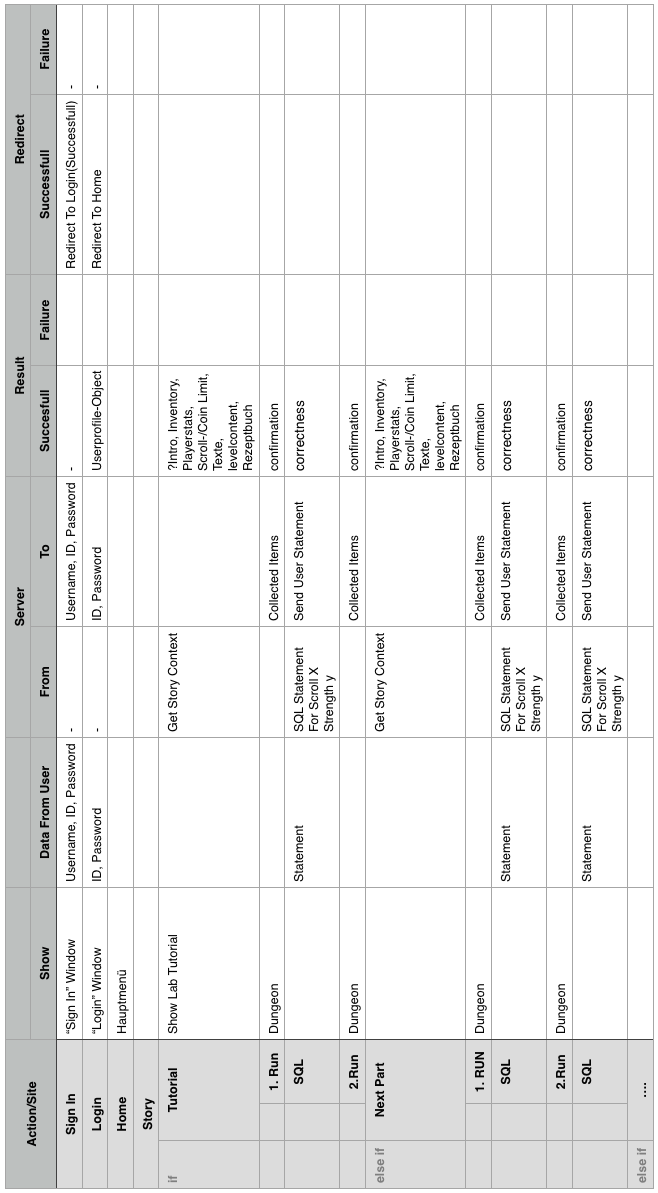
\includegraphics[width=0.75\textwidth]{figures/Spielablauf.PNG}
\caption{Veranschaulichung des Spielablaufes}
\end{figure}

\section{Trivia-Modus}
Der Trivia-Modus ist f\"ur die Spieler, die reines SQL lernen m\"ochten. Dazu kommt der SQL-Trainer zum Vorschein.   

W\"ahlt der Benutzer nun den „Trivia-Mode“ aus, so kann er SQL-Anfragen \"uben, ohne das Minispiel zu spielen. Geladen werden auch hier wieder, 
nach Anfrage durch das Front-End an das Back-End, s\"amtliche daf\"ur ben\"otigten Information. Diese bestehen demnach aus einem gesamten 
Task inklusive Datenbankschema und dem Anfragetext, zu welchem das SQL-Statement erstellt werden muss. Hierbei hat der Spieler von 
vornherein die M\"oglichkeit  einen aus f\"unf Schwierigkeitsgraden auszuw\"ahlen. Hat er sich f\"ur einen Schwierigkeitsgrad entschieden, beginnt 
der gleiche Ablauf, wie bei den Tasks im Story-Mode. Das Front-End schickt eine Anfrage an das Back-End und ein kompletter Task wird 
\"ubergeben. Aber auch in diesem Mode hat der Spieler die M\"oglichkeit, ohne Story-Content in das Dungeon zu gehen und nach Belieben mehr 
oder weniger viele, zuf\"allig ausgew\"ahlte, Maps zu spielen. Daf\"ur wird es einen eigens daf\"ur vorgesehenen Men\"upunkt  geben, mit dem der 
Spieler zu jeder Zeit hin, aber auch wieder zur\"uck wechseln kann.

\section{Shop}
Der Shop dient dazu, den Spielern ein wenig Raum f\"ur Personalisierung zu bieten. 
W\"ahlt der Benutzer „Shop“, wird ihm die M\"oglichkeit gegeben, gesammelte Lofi-Coins gegen Spieler-Avatare einzutauschen, die gleichzeitig die 
Spielfigur im Dungeon repr\"asentieren. Au{\ss}erdem soll es die M\"oglichkeit geben weitere Slots zum Belt der Spielfigur dazu zu kaufen. Auch
weitere Leben k\"onnen hier gegen Lofi-Coins erworben werden. 

\section{Hausaufgaben-Modus} 
W\"ahlt der Spieler „Homework“, so kann er die in der Applikation verkn\"upften Hausaufgaben bearbeiten. Hierbei stellt wieder das Front-End die 
Anfrage an das Back-End. Daf\"ur ist ein komplettes Aufgabenpaket mit unterschiedlich schwierigen SQL-Aufgaben vorgesehen. Die Hausaufgabe 
ist erst dann abgeschlossen, wenn das Aufgabenpaket unter einer bestimmten Abschlussbedingung erf\"ullt worden ist. Die Bedingung kann 
entweder ein Punkte-Limit oder ein Zeit-Limit sein. Ein Aufgabenpaket kann auch aus einer gewissen Anzahl an SQL-Statements bestehen.
Diese Bedingung kann von einem Wissenschaftlichen Mitarbeiter des Dozenten von RDBI f\"ur die w\"ochentlichen Challenges ausgew\"ahlt 
werden und in der Datenbank hinterlegt werden. Der Benutzer hat also nur innerhalb einer Woche Zeit das gesamte Aufgabenpaket zu l\"osen, 
erst dann wird die Hausaufgabe als abgeschlossen markiert.  Auch die Aufgabenstellung und die Statements der zu l\"osenden Aufgaben m\"ussen von dem 
Mitarbeiter in die Datenbank eingef\"ugt werden. Daf\"ur steht das Admin-Tool des Back-Ends zur Verf\"ugung. Ist ein Aufgabenpaket f\"ur eine 
bestimmte Woche erstellt worden, so kann sie von einem Studenten bearbeitet werden. W\"ahlt der Student die aktuelle Hausaufgabe aus, 
geht die Anfrage f\"ur eine erste Aufgabenstellung raus und das Back-End sendet die Aufgabe zur\"uck.

Schickt der Benutzer einmal ein Statement ab, so wird auch hier wieder eine Kontrolle durchgef\"uhrt und mit eventuellem Fehlerhinweis zur\"uckgeschickt. 
Der User korrigiert sein Statement und sendet es erneut an das Back-End. Bei richtiger Beantwortung wird dieses Statement als 
abgeschlossen markiert und auf dem Server gesichert. Bevor die Aufgaben jedoch gel\"ost werden k\"onnen, m\"ussen sie in das Back-End eingepflegt 
werden. Daf\"ur steht das Admin-Tool zur Verf\"ugung. Dort kann auch jeder Student nachschauen ob er die Hausaufgaben, beziehungsweise die 
Challenges, bestanden hat oder nicht.


\section{Admin-Tool}
Das Admin-Tool stellt f\"ur verschiedene Benutzergruppen unterschiedliche Funktionen zur Verf\"ugung. Studenten, die sich mit ihrer y-Nummer registriert haben,
k\"onnen hier die Ergebnisse aller von ihnen bearbeiteten Hausaufgaben einsehen. Wenn ein Spieler die vom Kunden gew\"unschten Kriterien erf\"ullt hat, k\"onnen 
diese „bef\"ordert“ werden. Einem bef\"orderten Benutzer ist es m\"oglich selbst Aufgaben zu erstellen, die von anderen Spielern im Trivia-Mode bearbeitet werden k\"onnen, 
wenn sie diese Funktion wahrnehmen m\"ochten. Dieses kann jeder Spieler f\"ur sich entscheiden und im Men\"u im Trivia-Mode die daf\"ur vorgesehene Checkbox aktivieren.
Des Weiteren gibt es die Gruppe der Administratoren. Diese sind vor allem f\"ur die Benutzerverwaltung verantwortlich. Sie k\"onnen Benutzer l\"oschen, Challenge-Pakete 
und Hausaufgaben erstellen, sowie die L\"osungen der Studenten einsehen.

\section{Einstellungen}
Wählt der Benutzer „Settings“ hat er Zugriff auf allgemeine Einstellungen. Diese werden Spieler-spezifisch im Back-End gespeichert und beim Aufruf 
von diesem erfragt. Der User hat nun die folgenden Einstellungsmöglichkeiten:
\begin{itemize}	
	\item Sound on/off: Aktiviert oder deaktiviert die Soundeffekte die beim Springen der Spielfigur oder beim Bet\"atigen eines Buttons abgespielt werden.
	\item Music on/off: Aktiviert oder deaktiviert die Hintergrundmusik des Minispiels.
	\item Tutorial: Das Tutorial kann reaktiviert werden, damit die Spieler, die es vermeidlich \"ubersprungen haben, dieses trotzdem nochmal ansehen k\"onnen. 
	\item Story-Reset: Setzt den Fortschritt des Story-Modes nach zurück. Dieses muss best\"atigt werden.
	\item Change Username: Gibt dem User die Möglichkeit, seinen Benutzernamen zu ändern.
	\item Change Password: Gibt dem User die Möglichkeit, sein Passwort zu ändern.
	\item Delete Profile: Hiermit kann der User sein komplettes Profil l\"oschen.
\end{itemize}	
Erfolgt eine Änderung der Einstellungen, wird diese sofort ans Back-End geschickt, dort gespeichert und kurz darauf im Front-End aktualisiert.
	
	
\section{Ranglisten}
Die Leaderboards dienen zus\"atzlich zu dem Minispiel als Motivationsf\"orderung.
Wählt der Benutzer „Leaderboards“ bekommt er eine Einsicht in Ranglisten, in denen die Statistiken aller Benutzer in den verschiedenen Modi dargestellt werden.
Folgende Ranglisten gibt es sowohl für den „Story-Mode“ als auch für den „Trivia-Mode“:
\begin{itemize}	
	\item Gesamtanzahl Lofi-Coins (total lofi-coins)
	\item Gesamtanzahl Läufe (total runs)
	\item geringsten Anzahl an benötigten Durchgängen für die Story (min. runs per story)
	\item insgesamt im Spiel verbrachten Zeit (time spent)
	\item Anzahl an abgeschlossenen Stories (story count)
	\item prozentuale Erfolgsquote beim Beantworten von Anfragen
	\item prozentuale Erfolgsquote der beim ersten Versuch korrekt beantworteten Anfragen
\end{itemize}
	
Die „Top Ten“ jeder dieser Ranglisten werden direkt als Liste dargestellt. Ist der Benutzer unter diesen, wird er markiert, falls nicht, wird sein Rang unter dieser 
Liste angezeigt. Der Benutzer hat die Möglichkeit sowohl seinen eigenen Rang, als auch den anderer Benutzer zu sehen, sofern er deren Benutzernamen kennt. 
Die Daten für die Ranglisten werden vom Back-End zusammengestellt und auf Anfrage ans Front-End gesendet.


\section{Musskriterien}\label{sec:musskriterien}
\must{1}{Es wird ein „Jump\&Run“-Minispiel f\"ur die Motivationsf\"orderung der User geben.}
\must{2}{Ein grafisch aufbereitetes Webinterface, in dem die Men\"uf\"uhrung eingebettet ist.}
\must{3}{Ein SQL-Trainer, das aus einem Aufgabenstellungsfenster und einem Eingabefenster besteht.}
\must{4}{Das Back-End wird entsprechende Nutzerdaten der Spieler speichern, sichern.}
\must{5}{Das Back-End wird ein Admin-Tool zur Userverwaltung zur Verf\"ugung stellen.}
\must{6}{Das Back-End wird ein Admin-Tool zur Aufgabenverwaltung zur Verf\"ugung stellen.}
\must{7}{Es wird die drei verschiedenen Spielmodi geben (Trivia-, Story und Homework-Mode).}
\must{8}{Die Software wird an das LDAP der Technischen Universit\"at Braunschweig angebunden.}
\must{9}{Die Game-Engine ist in das Back-End integriert.}


\section{Sollkriterien}\label{sec:sollkriterien}
\should{1}{Das Minispiel kann in verschiedenen Schwierigkeitsgraden gespielt werden.}
\should{2}{Die Applikation soll auf mobilen Endger\"aten ausf\"uhrbar sein.}
\should{3}{Der Avatar, beziehungsweise die Spielfigur sollen ersetzt oder personalisiert werden k\"onnen.}
\should{4}{Es k\"onnen Highscores generiert und im Profil visualisiert werden.}
\should{5}{Auch Leaderboards sollen generiert und in einem eigenen Men\"upunkt visualisiert werden k\"onnen.}


\section{Kannkriterien}\label{sec:kannkriterien}
\could{1}{Es k\"onnten neben den Hausaufgaben-Paketen auch \"Ubungspakete erstellt werden k\"onnen.}
\could{2}{Auch andere Universit\"aten k\"onnten \"uber ein entspechendes LDAP angebunden werden.}
\could{3}{Es k\"onnte ein abgespecktes Tutorial f\"ur den Trivia-Mode geben.}
\could{4}{In den Shop k\"onnten weitere Features integriert werden.} 
\could{5}{Die Steuerung des Minispiel kann auf Tasten, statt Mausklicks gelegt werden.}
\could{6}{Es soll Freundeslisten geben k\"onnen.}


\section{Abgrenzungskriterien}\label{sec:abgrenzungskriterien}
\wont{1}{Die Verkn\"upfung zu Social-Networks soll nicht realisiert werden.}
\wont{2}{Es wird keinen Mode geben, in dem der Fokus nur auf dem Minispiel liegt.}
\wont{3}{Innerhalb der Applikation wird es keine M\"oglichkeit f\"ur In-Game-K\"aufe geben.}
\wont{4}{Es wird keine kostenpflichtigen Zugriffsm\"oglichkeiten f\"ur die Software geben.}
\wont{5}{Es werden keine Hausaufgabenergebnisse in das HMS des Instituts f\"ur Informationssysteme \"ubertragen.}
%!TEX root = ../Pflichtenheft.tex

\chapter{Produkteinsatz}

\section{Anwendungsbereiche}
The SQL Alchemist wird entwickelt, um den Umgang und das praktische Anwenden von SQL-Anfragen einfach und spielerisch üben, beziehungsweise lernen zu können.
Dies ist oftmals nicht ohne Weiteres möglich, da es ein großer Aufwand ist sich selbst einen Datenbankserver zu installieren, ihn mit Daten und eigenem geeigneten Schema 
zu füllen und sich dafür eigene Aufgaben auszudenken, sowie diese auf Korrektheit zu überprüfen.
Die Anwendung wird nicht explizit Bezug auf die Vorlesung nehmen, sondern weitestgehend autonom funktionieren, mit Ausnahme des „Homework-Mode“, der durch die 
Wissenschaftlichen Mitarbeiter der TU Braunschweig genutzt werden kann, um den Studenten der RDB1-Vorlesung SQL-Hausaufgaben zu stellen.
Dieser Modus ist nur durch die Anmeldung als Student mit bekannter y-Nummer erreichbar.

\section{Zielgruppen}
Die Studenten der TU Braunschweig sind die Hauptzielgruppe. Um das Modul „RDB1“ erfolgreich abzuschließen ist es notwendig, die geforderten Pflichthausaufgaben im 
Homework-Mode zu absolvieren. Damit die Studenten motivierter lernen können, enthält der Story-Modus ein „Jump\&Run“-Minigame. 
Will sich der Student jedoch optimal auf die Klausur vorbereiten, um die SQL-Anfragen zu vertiefen, ist es hilfreich so viel wie möglich zu üben. 
Dies ist durch den Trivia-Mode möglich, in dem der Spieler Aufgaben in verschiedenen, wählbaren Schwierigkeitsgraden bearbeiten kann.

Auch für die wissenschaftlichen Mitarbeiter ist die Anwendung von Nutzen. Die gestellten Hausaufgaben müssen nicht mehr von Hand einzeln kontrolliert werden, 
da die Hausaufgaben in der Anwendung selbst geprüft und automatisch als abgeschlossen markiert werden, wenn alle Aufgabenteile korrekt bearbeitet wurden.
Sie müssen so nur die wöchentlichen Aufgaben in die Datenbank eintragen.

Für die Professoren ist die Anwendung insofern interessant, dass sie einen neuen Weg darstellt, um die Studenten für etwas sehr theoretisches, aber vorlesungsrelevantes 
zu begeistern und ihnen so eine motivierende Möglichkeit geboten wird, diese wichtigen Fähigkeiten auf angenehme Weise zu verinnerlichen. Da SQL aber nicht nur an der 
Universität wichtig ist, sondern vor allem in der Arbeitswelt eine wesentliche Rolle spielt, spricht die Anwendung auch private Nutzer an. Diese können ihr Wissen auf diesem 
Gebiet erweitern und festigen oder sogar völlig neu zu erlernen.
Neue Nutzer, also keine Studenten, können sich mit ihrer E-Mail-Adresse anmelden. Für diese Gruppe fällt der Homework-Mode weg und ist somit nicht nutzbar. Eventuell 
könnte die Anwendung später auch von anderen Universitäten in ihrem Vorlesungsbetrieb unterstützend eingesetzt werden.
Das Minispiel ist nur in Verbindung mit dem Lernen verwendbar. Ein Einzelmodus nur für das Minispiel gibt es nicht.


\section{Betriebsbedingungen}
Um die Anwendung nutzen zu können, wird ein internetfähiges Endgerät mit installiertem Webbrowser benötigt, zum Beispiel ein Computer, Smartphone oder Tablet.
Durch die Plattformunabhängigkeit kann sie auch unterwegs auf dem Smartphone verwendet werden.
Da es zudem keine App ist, die auf das Gerät geladen werden muss, sind keine manuellen Aktualisierungen durch den Benutzer nötig. Alle Updates können durch die 
Administratoren durchgeführt werden, ohne dass sie erst durch eine Handlung des Nutzers wirksam gemacht werden müssen.
Der Homework-Mode erfordert während des Semesters wöchentliche Betreuung durch einen wissenschaftlichen Mitarbeiter, der die aktuellen Aufgaben in die Datenbank einfügt.
Auch die Serverapplikation, sprich das Admin-Tool, ist \"uber einen einfachen Internetbrowser erreichbar.



%!TEX root = ../Pflichtenheft.tex

\chapter{Produktübersicht}



\section{Die Registration}


\begin{figure}[ht]
\centering
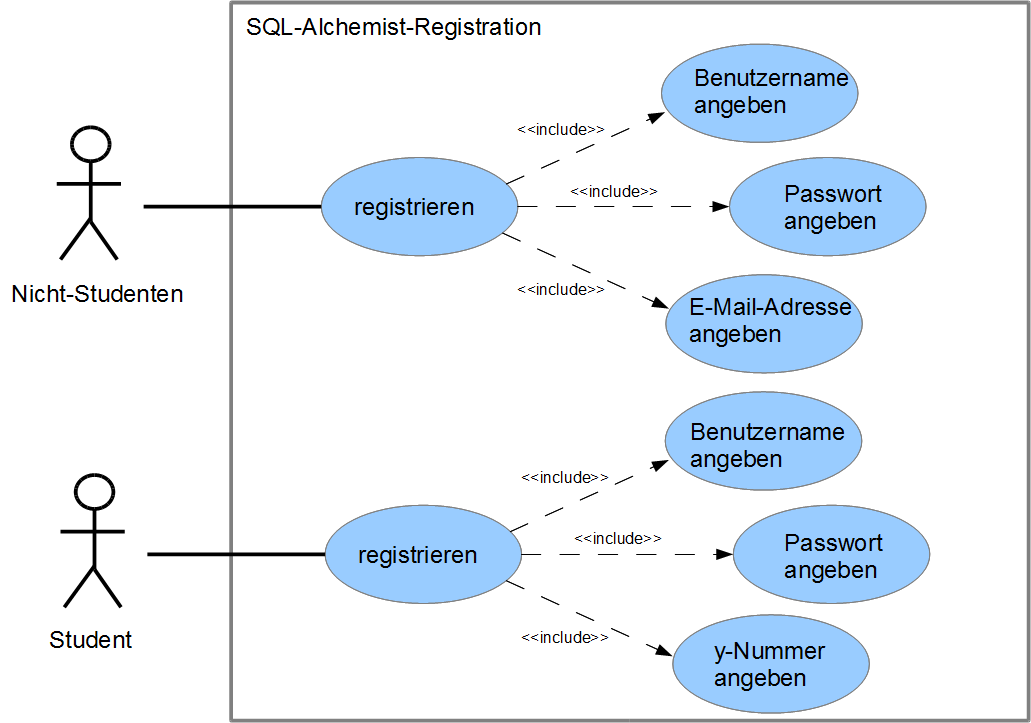
\includegraphics[width=1.0\textwidth]{figures/Registration.PNG}
\caption{Die Registration}
\end{figure}\\
In diesem Use-Case-Diagramm werden die Abl\"aufe aus Nutzersicht beschrieben, die zur Registration nötig sind. Dabei muss zwischen Studenten und Nicht-Studenten unterschieden werden.
Studenten müssen zur Registration ihre y-Nummer, einen Benutzernamen und das zu ihrer y-Nummer gehörige Passwort angeben.\\
Nicht-Student müssen zur Registration eine E-Mail-Adresse, einen Benutzernamen und ein Passwort angeben.\\\\\\\\\\




\begin{figure}[ht]
\centering
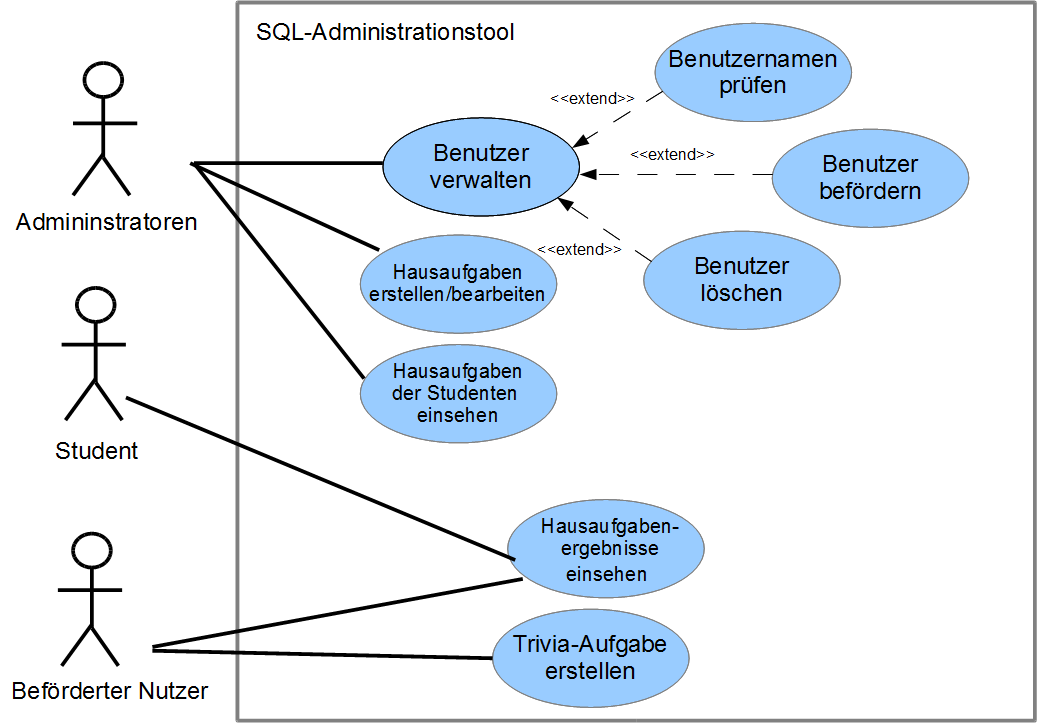
\includegraphics[width=0.8\textwidth]{figures/Admintool.PNG}
\caption{Das Admintool}
\end{figure}\\
In diesem Use-Case-Diagramm ist zu sehen, welche Möglichkeiten das Admin-Tool bereit stellt. Dabei gibt es verschiedene Nutzergruppen mit verschiedenen Rechten. 
Externe registrierte Benutzer haben standardmäßig keinen Zugriff auf das Admin-Tool.\\
Registrierte Studenten können im Admin-Tool einsehen, wie sie in ihren Hausaufgaben abgeschnitten haben. Das schließt sowohl die aktuellen, als auch die voran gegangenen ein.
Beförderte Benutzer haben, zusätzlich zu ihren Standardfunktionen (externe keine, Studenten Hausaufgaben-Übersicht) weiterhin die Möglichkeit, selber Aufgaben/ -pakete zuerstellen und die erstellten Aufgaben von anderen beförderten Benutzern zu bewerten.\\
Administratoren erhalten die Rechte zur Nutzer-, Inhalts- und Hausaufgabenverwaltung.  \\\\\\\\\\





\section{Der Story-Mode}
Das folgende Aktivit\"atsdiagramm zeigt detailliert den Ablauf der Story. Um die Story zu spielen loggt sich der User ein und w\"ahlt im Hauptmen\"u den Reiter
\glqq Story\grqq~aus. An diesem Punkt hat er bereits die M\"oglichkeit sich umzuentscheiden. M\"ochte er tats\"achlich die Story spielen, so gelangt man in das 
so genannte Laboratory, w\"ahlt ein Rezept bzw. Scroll aus und braut sich seinen gew\"unschten Trank, indem er via SQL -Statement die daf\"ur gebrauchten 
Materialien aus dem Schrank \glqq Secreterry\grqq~anfordert.
Anschlie{\ss}end hat er die M\"oglichkeit entweder aus dem Story-Modus rauszugehen oder das Minispiel im Dungeon zu starten. Dort muss er alle  H\"urden 
\"uberwinden und kann sich dann dazu entscheiden den Prozess des Trankbrauens zu wiederholen oder den Modus zu verlassen.
\begin{figure}[ht]
\centering
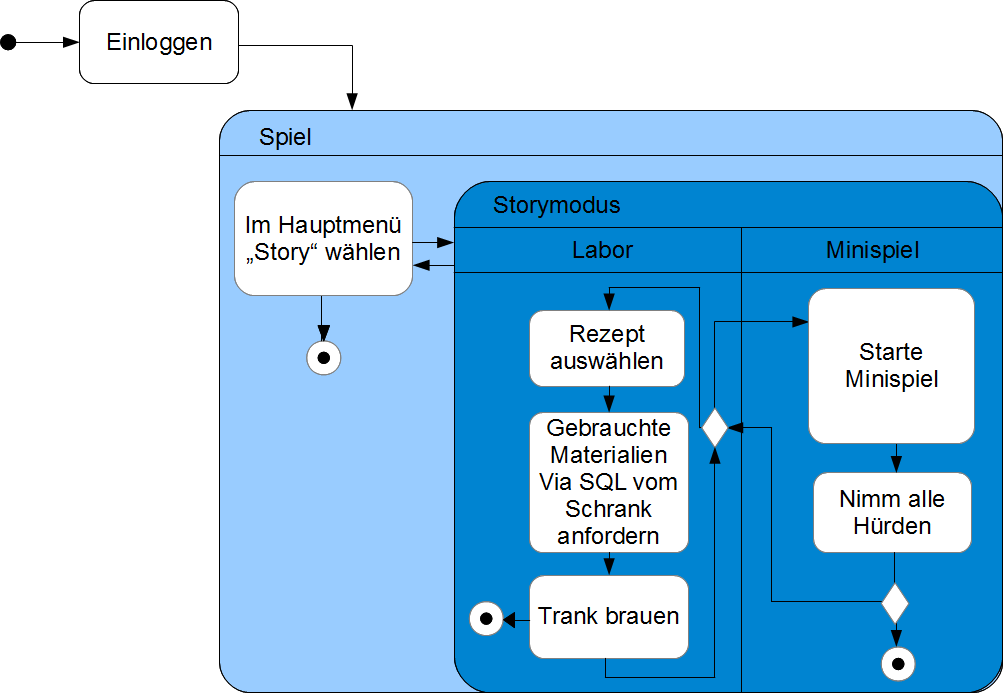
\includegraphics[width=1\textwidth]{figures/story_mode_activ.PNG}
\caption{Spielablauf im Story-Modus}
\end{figure}





\section{Das Spiel}
Im folgenden Aktivit\"atsdiagramm ist der Vorgang des Logins und der Registration beschrieben.
Nach dem Spielstart ist der Login-Bildschirm zusehen. 
Ist der Nutzer noch nicht registriert kann er dies, nach Druck auf den \glqq Sign up\grqq~Knopf, tun.
Hier muss er, je nach dem ob er Student ist oder nicht, entweder seine y-Nummer, das dazugeh\"orige Passwort, oder eine E-Mail-Adresse und ein selbst ausgedachtes 
Passwort angeben. Dazu geh\"ort in beiden F\"allen noch ein Benutzername. Nach erfolgreicher Registrierung wird man in das Hauptmen\"u weitergeleitet.\\
Sind E-Mail-Adresse, bzw. y-Nummer, und Passwort schon registriert, kann man diese im Login-Bildschirm angeben und gelang danach ins Hauptmen\"u. Der 
Benutzername wird f\"ur den Login-Vorgang nicht ben\"otigt.
\begin{figure}[ht]
\centering
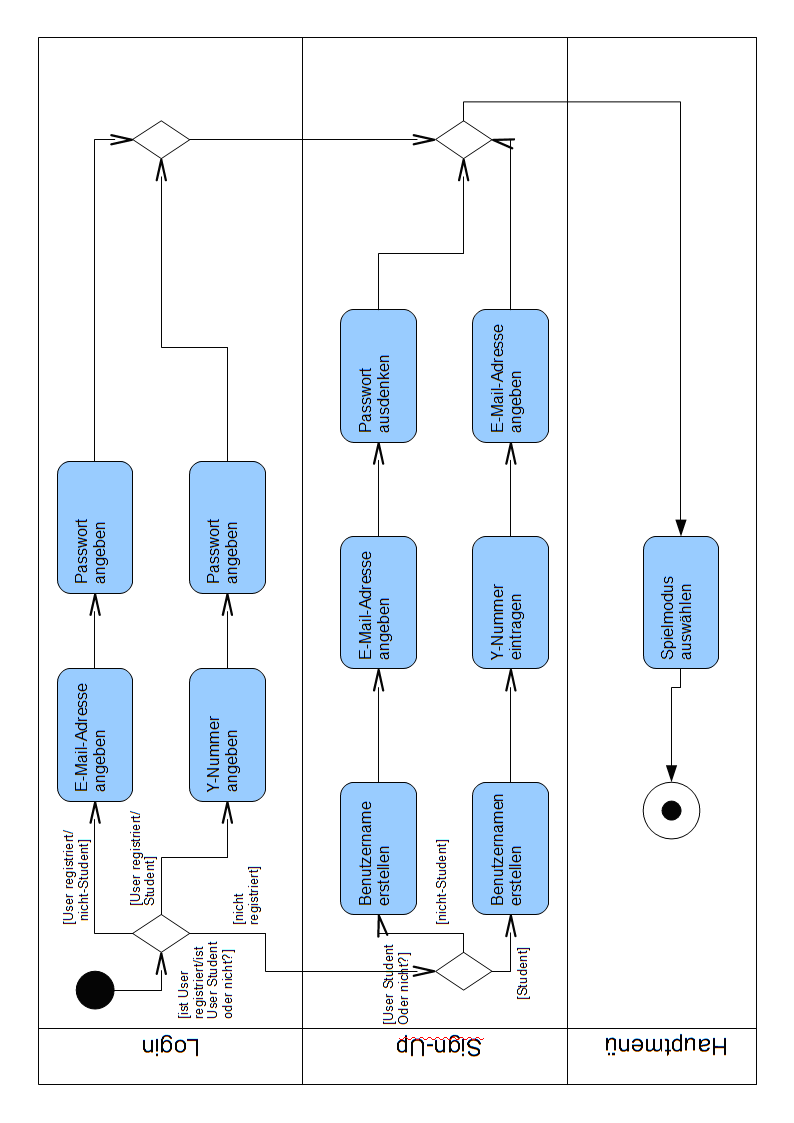
\includegraphics[width=1\textwidth]{figures/aktiv_RegLog.PNG}
\caption{Login-/Registrationsvorgang}
\end{figure}


\begin{figure}[ht]
\centering
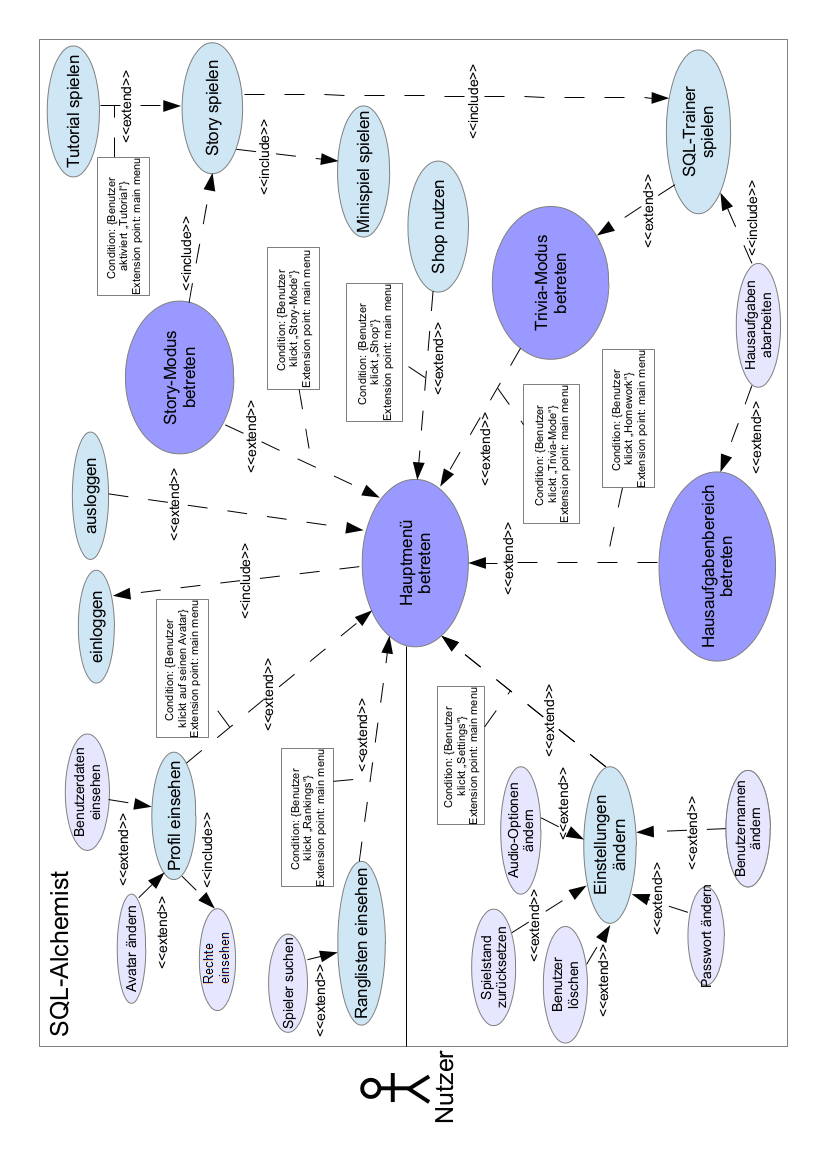
\includegraphics[width=1\textwidth]{figures/UseCaseDiagrammFinal.PNG}
\caption{Der Großteil des eigentlichen Spiels}
\end{figure}
Das folgende Use-Case-Diagramm  zeigt den Gro{\ss}teil des Spielablaufs. Loggt sich der User ein, so gelangt er in das Hauptmen\"u. In diesem Men\"u 
hat er verschiedene M\"oglichkeiten zu interagieren. Zum einen kann er sein Profil einsehen. Dort hat er die Option sowohl seinen Avatar zu \"andern, als auch seine 
Benutzerdaten einzusehen. M\"ochte der User wissen welche Nutzerrechte er hat, so kann er dies ebenfalls dort tun.
Zum anderen kann der User unterschiedliche Ranglisten einsehen, andere Spieler suchen und sich deren Rang anzeigen lassen.

Eine weitere M\"oglichkeit in dem Men\"u voranzuschreiten, ist die, pers\"onliche Einstellungen zu ver\"andern. Diese sind: 
\begin{itemize}
	\item Der User kann Audio-Optionen \"andern.
	\item Er kann seinen Spielstand zur\"ucksetzen.
	\item Er hat auch die M\"oglichkeit sein Profil komplett zu l\"oschen.
	\item Er kann sein Passwort \"andern.
	\item Er kann seinen Benutzernamen l\"oschen.
\end{itemize}

Au{\ss}erdem kann der User im Shop unterschiedliche Erweiterungen f\"ur sein Spielfigur erwerben.

Des Weiteren kann der Benutzer einen von drei verschiedene Spiel-Modi w\"ahlen. Diese sind alle untereinander verkn\"upft. Betritt der Spieler den 
Hausaufgaben-Modus, so kann er dort, die von einem Wissenschaftlichen Mitarbeiter des Dozenten der Vorlesung RDB1 gestellten Aufgaben l\"osen. 
M\"ochte man diese bearbeiten, so schlie{\ss}t das die Benutzung des SQL-Trainers ein. Dieser ist ebenfalls aus dem Trivia-Modus erreichbar. Der Trainer
ist auch fester Bestandteil des Story-Modes. M\"ochte der User die Story spielen, so impliziert das ebenfalls das Spielen des Minispiels.
Im Story-Modus ist dabei die M\"oglichkeit gegeben, vor Start der eigentlichen Story, ein Tutorial zu absolvieren. Dieses ist hierbei aber eine freiwillige Option.

Die letzte Option die sich im Hauptmen\"u noch bietet, ist die, sich auszuloggen.




%!TEX root = ../Pflichtenheft.tex

% Kapitel 4
%-------------------------------------------------------------------------------

\chapter{Produktfunktionen}\label{test1}

\section{Nutzer registrieren}
\begin{function}{10}{Nutzer registrieren}
\item[Anwendungsfall:] Ein neuer Benutzer möchte Zugang zum Spiel erhalten.
\item[Anforderung:] \ref{RM4}, \ref{RM8}, \ref{RC2}
\item[Ziel:] Der Benutzer wird registriert und erhält eigene Login-Daten.
\item[Vorbedingung:] Der Nutzer ist noch nicht registriert.
\item[Nachbedingung Erfolg:] Der Nutzer verfügt über eigene eindeutige Login-Daten und wird zum Login-Bereich weitergeleitet.
\item[Nachbedingung Fehlschlag:] Die eingegebenen Daten waren nicht vollständig und die Registrierung schlägt fehl; es wird eine entsprechende Fehlermeldung angezeigt.
\item[Akteure:] ~Nutzer und Programm
\item[Auslösendes Ereignis:] Der Nutzer hat die zum Spiel gehörende URL eingegeben und klickt auf „Sign Up“.
\item[Beschreibung:] ~
\begin{enumerate}
  \item  Der Nutzer gibt in die vorgesehenen Texteingabefelder einen Benutzernamen, ein Passwort, sowie eine E-Mail-Adresse oder y-Nummer ein.
  \item  Der Nutzer bestätigt seine Eingaben mit einem Klick auf einen Button.
  \item Verfügt der Nutzer über eine y-Nummer, so ist er automatisch verifiziert, andernfalls erhält er eine E-Mail mit einem Aktivierungslink, den er zur Verifikation anklicken muss.
  \item  Der Nutzer wird anschließend zum Login-Bereich weitergeleitet.
\end{enumerate}
\end{function}

\section{Nutzer anmelden}
\begin{function}{20}{Nutzer anmelden}
\item[Anwendungsfall:] Einloggen des Nutzers um Zugang zum Spiel zu erhalten.
\item[Anforderung:] \ref{RM8}, \ref{RC2}
\item[Ziel:] Der Nutzer wird angemeldet.
\item[Vorbedingung:] Der Nutzer muss sich registriert und dadurch einen Account erstellt haben.
\item[Nachbedingung Erfolg:]  Die eingegebenen Daten wurden als korrekt verifiziert und der Nutzer wird auf den Hauptbildschirm weitergeleitet.
\item[Nachbedingung Fehlschlag:] Die eingegebenen Daten waren nicht korrekt und dem Nutzer wird der Zugang verweigert; es wird eine entsprechende Fehlermeldung angezeigt.
\item[Akteure:] ~Nutzer und Programm
\item[Auslösendes Ereignis:] Der Nutzer hat die zum Spiel gehörende URL eingegeben und wurde zum Login-Bildschirm weitergeleitet.
\item[Beschreibung:] ~
\begin{enumerate}
  \item  Der Nutzer gibt seine Email-Adresse/y-Nummer in das dafür vorgegebene Feld ein.
  \item  Der Nutzer gibt sein Passwort in das dafür vorgesehene Feld ein.
  \item Der Nutzer klickt auf „Einloggen“.
  \item  Das System gleicht die eingegebenen Daten mit den Nutzerdaten in der Datenbank ab.
  \item Der Nutzer wird zum Hauptbildschirm weitergeleitet.
\end{enumerate}
\end{function}

\section{Nutzer abmelden}
\begin{function}{30}{Nutzer abmelden}
\item[Anwendungsfall:] Der Nutzer will das Spiel verlassen und sich abmelden.
\item[Anforderung:] -
\item[Ziel:] Der Nutzer wird abgemeldet.
\item[Vorbedingung:] Der Nutzer muss sich im Hauptmenü befinden.
\item[Nachbedingung Erfolg:]  Die Abmeldung ist erfolgt und der Nutzer wird zum Anmeldebereich weitergeleitet. Ohne erneute Anmeldung ist keine Aktivität im Spiel mehr möglich.
\item[Nachbedingung Fehlschlag:] Es gab einen Fehler beim Ausführen der Abmeldung und eine entsprechende Meldung wird ausgegeben.
\item[Akteure:] ~Nutzer und Programm
\item[Auslösendes Ereignis:] Der Nutzer hat im Hauptmenü auf den „Logout“-Button geklickt.
\item[Beschreibung:] ~
\begin{enumerate}
  \item  Der Nutzer wird abgemeldet und verlässt das Spiel
\end{enumerate}
\end{function}

\section{Profil einsehen}
\begin{function}{40}{Profil einsehen}
\item[Anwendungsfall:] Der Nutzer möchte seine bisher gemachten Fortschritte nachverfolgen und ruft zu diesem Zweck sein Profilfenster auf.
\item[Anforderung:] \ref{RM2}, \ref{RM4}, \ref{RS4}, \ref{RS5}
\item[Ziel:] Der Nutzer kann sein Profil einsehen.
\item[Vorbedingung:] Der Nutzer muss sich eingeloggt haben.
\item[Nachbedingung Erfolg:]  Dem Nutzer wird sein Profilfenster, in welchem dessen Fortschritte in Form von Statistiken festgehalten werden, angezeigt.
\item[Nachbedingung Fehlschlag:] Es gab einen Fehler beim Aufruf und eine entsprechende Meldung wird ausgegeben.
\item[Akteure:] ~Nutzer und Programm
\item[Auslösendes Ereignis:] Der Nutzer hat auf seinen Avatar geklickt.
\item[Beschreibung:] ~
\begin{enumerate}
  \item  Das Profilfenster wird geöffnet
  \item  Der Nutzer sieht seine Statistiken und Nutzerdaten ein.
\end{enumerate}
\end{function}

\section{Benutzernamen \"andern}
\begin{function}{50}{Benutzernamen ändern}
\item[Anwendungsfall:] Der Nutzer will seinen Benutzernamen ändern.
\item[Anforderung:] \ref{RM4}
\item[Ziel:] Der Benutzername, der im Spiel und in den Ranglisten verwendet wird, wird geändert.
\item[Vorbedingung:] Der Nutzer muss sich eingeloggt haben und sich im „Settings“-Menü befinden.
\item[Nachbedingung Erfolg:]  Dem Nutzer wird sein Profilfenster mit dem neuen Benutzernamen angezeigt.
\item[Nachbedingung Fehlschlag:] Es gab einen Fehler beim Ändern des Benutzernamens und eine entsprechende Meldung wird ausgegeben. Der Nutzer behält seinen alten Nutzernamen.
\item[Akteure:] ~Nutzer und Programm
\item[Auslösendes Ereignis:] Der Nutzer klickt auf den „Change Username“-Button.
\item[Beschreibung:] ~
\begin{enumerate}
  \item  Es öffnet sich ein Texteingabefenster, in dem der Nutzer seinen neuen Benutzernamen eingibt.
  \item  Er bestätigt seine Eingabe, anschließend prüft das Programm, ob der Benutzername verwendet werden darf (also noch nicht vergeben ist).
\end{enumerate}
\end{function}

\section{Passwort \"andern}
\begin{function}{60}{Passwort ändern}
\item[Anwendungsfall:] Ein Nutzer will sein Passwort ändern.
\item[Anforderung:] \ref{RM6}
\item[Ziel:] Das Passwort wird geändert.
\item[Vorbedingung:] Der Nutzer muss eingeloggt sein und sich im „Settings“-Menü befinden.
\item[Nachbedingung Erfolg:]  Der Nutzer hat sein neues Passwort zugewiesen bekommen und gelangt zurück ins „Settings“-Menü.
\item[Nachbedingung Fehlschlag:] Es gab einen Fehler und eine entsprechende Meldung wird ausgegeben. Der Nutzer behält sein bisheriges Passwort.
\item[Akteure:] ~Nutzer und Programm
\item[Auslösendes Ereignis:] Der Nutzer klickt im „Settings“-Menü auf den Button „Change Password“
\item[Beschreibung:] ~
\begin{enumerate}
  \item  Es öffnet sich ein Texteingabefeld, in das der Nutzer das neue Passwort eingibt.
  \item  Der Benutzer muss sein altes Passwort zur Verifikation in einem weiteren Texteingabefeld eingeben.
  \item Der Nutzer bestätigt seine Eingaben.
\end{enumerate}
\end{function}

\section{Avatar \"andern}
\begin{function}{70}{Avatar ändern}
\item[Anwendungsfall:] Ein Nutzer will seinen Avatar (Spielfigur) ändern.
\item[Anforderung:]\ref{RM4}, \ref{RS3}
\item[Ziel:] Der Avatar des Nutzers wird geändert.
\item[Vorbedingung:] Der Nutzer muss eingeloggt sein und sich im „Profile“-Menü befinden.
\item[Nachbedingung Erfolg:]  Der neue Avatar des Nutzers wird übernommen.
\item[Nachbedingung Fehlschlag:] Es gab einen Fehler und eine entsprechende Meldung wird ausgegeben. Der Nutzer behält seinen bisherigen Avatar.
\item[Akteure:] ~Nutzer und Programm
\item[Auslösendes Ereignis:] Der Nutzer klickt im „Profile“-Menü auf den Button „Change Avatar“.
\item[Beschreibung:] ~
\begin{enumerate}
  \item  Es wird eine Liste angezeigt, die alle möglichen Avatare enthält.
  \item  Der Nutzer wählt einen Avatar aus der Liste aus.
  \item Die Auswahl wird über einen Button bestätigt.
\end{enumerate}
\end{function}

\section{Benutzer l\"oschen}
\begin{function}{80}{Benutzer löschen}
\item[Anwendungsfall:] Ein Nutzer will seinen Account löschen.
\item[Anforderung:] \ref{RM4}, \ref{RM5}
\item[Ziel:] Der Nutzeraccount wird gelöscht.
\item[Vorbedingung:] Der Nutzer muss eingeloggt sein und sich im „Settings“-Menü befinden.
\item[Nachbedingung Erfolg:]  Der Account des Nutzers wurde, inklusive aller auf diesen bezogenen Daten (ausgenommen die von diesem Nutzer erstellten SQL-Abfragen), aus der Nutzerverwaltung gelöscht. Der Nutzer wird automatisch ausgeloggt.
\item[Nachbedingung Fehlschlag:] Es gab einen Fehler und eine entsprechende Meldung wird ausgegeben. Der Account bleibt unverändert.
\item[Akteure:] ~Nutzer und Programm
\item[Auslösendes Ereignis:] Der Nutzer klickt im „Settings“-Menü auf den Button „Delete User“.
\item[Beschreibung:] ~
\begin{enumerate}
  \item  Der Nutzer wird gefragt, ob er wirklich seinen Account löschen möchte.
  \item  Der Nutzer bestätigt sein Vorhaben und  sein Account wird gelöscht, außerdem wird er automatisch ausgeloggt.
\end{enumerate}
\end{function}

\section{Audioeinstellungen bearbeiten}
\begin{function}{90}{Audioeinstellungen bearbeiten}
\item[Anwendungsfall:] Ein Nutzer will die  Soundeffekte oder die Musik aktivieren/deaktivieren.
\item[Anforderung:] -
\item[Ziel:] Die Audioeinstellungen werden geändert.
\item[Vorbedingung:] Der Nutzer muss eingeloggt sein und sich im „Settings“-Menü befinden.
\item[Nachbedingung Erfolg:]  Die Audioeinstellungen wurden geändert und deren Status wurde im Back-End gespeichert.
\item[Nachbedingung Fehlschlag:] Es gab einen Fehler und eine entsprechende Meldung wird ausgegeben. Die bisherigen Einstellungen bleiben bestehen.
\item[Akteure:] ~Nutzer und Programm
\item[Auslösendes Ereignis:] Der Nutzer klickt im „Settings“-Menü auf den Button „Audio Settings“.
\item[Beschreibung:] ~
\begin{enumerate}
  \item  Es öffnet sich ein Fenster, in dem der Nutzer die Soundeffekte und die Musik unabhängig voneinander an- und abschalten kann. 
  \item  Der Nutzer bestätigt die Änderungen.
\end{enumerate}
\end{function}

\section{Spielstand zurücksetzen}
\begin{function}{100}{Spielstand zurücksetzen}
\item[Anwendungsfall:] Ein Nutzer möchte das Spiel erneut von vorne beginnen.
\item[Anforderung:] -
\item[Ziel:] Der Spielstand wird zurückgesetzt.
\item[Vorbedingung:] Der Nutzer muss eingeloggt sein und sich im „Settings“-Menü befinden.
\item[Nachbedingung Erfolg:]  Der Spielstand ist zurückgesetzt.
\item[Nachbedingung Fehlschlag:] Es gab einen Fehler und eine entsprechende Meldung wird ausgegeben. Der bisherige Speicherstand bleibt bestehen.
\item[Akteure:] ~Nutzer und Programm
\item[Auslösendes Ereignis:] Der Nutzer klickt im „Settings“-Menü auf den Button „Reset Story“.
\item[Beschreibung:] ~
\begin{enumerate}
  \item  Der Nutzer wird gefragt, ob er wirklich seinen Spielstand zurücksetzen möchte.
  \item  Der Nutzer bestätigt das Löschen.
\end{enumerate}
\end{function}

\section{Tutorial spielen}
\begin{function}{110}{Tutorial spielen}
\item[Anwendungsfall:] Ein Nutzer startet den "`Story-Mode"´.
\item[Anforderung:] -
\item[Ziel:] Der Nutzer lernt die Grundsteuerung des Spieles kennen.
\item[Vorbedingung:] Der Nutzer muss eingeloggt sein und den "`Story-Mode"´ gestartet haben. Außerdem muss das Tutorial aktiviert sein.
\item[Nachbedingung Erfolg:]  Der Nutzer hat das Tutorial erfolgreich absolviert und der Anfang der Story wird gestartet.
\item[Nachbedingung Fehlschlag:] Es gab einen Fehler und das Tutorial konnte nicht gestartet werden.
\item[Akteure:] ~Nutzer und Programm
\item[Auslösendes Ereignis:] Der Nutzer startet den „Story-Mode“.
\item[Beschreibung:] ~
\begin{enumerate}
  \item  Das Tutorial wird gestartet.
  \item  Der Nutzer erhält Anweisungen, die dieser befolgen muss.
  \item Nach Abschluss aller Aufgaben wird das Tutorial abgeschlossen.
\end{enumerate}
\end{function}

\section{Story spielen}
\begin{function}{120}{Story spielen}
\item[Anwendungsfall:] Ein Nutzer möchte den „Story-Mode“ spielen. 
\item[Anforderung:] \ref{RM7}
\item[Ziel:] Der Nutzer spielt die Story.
\item[Vorbedingung:] Der Nutzer muss eingeloggt sein und sich im Hauptmenü befinden.
\item[Nachbedingung Erfolg:]  Der Nutzer spielt den „Story-Mode“ bis er von selbst abbricht oder die Story bis zum Ende absolviert hat.
\item[Nachbedingung Fehlschlag:] Es gab einen Fehler und die Story konnte nicht gestartet werden. Eine entsprechende Meldung wird ausgegeben.
\item[Akteure:] ~Nutzer und Programm
\item[Auslösendes Ereignis:] Der Nutzer klickt im Hauptmenü auf den Button „Story-Mode“.
\item[Beschreibung:] ~
\begin{enumerate}
  \item  Der Story-Durchlauf wird gestartet.
  \item  Der Nutzer spielt die Story, bis er sie zu einem beliebigen Zeitpunkt abbricht.
\end{enumerate}
\end{function}

\section{SQL-Trainer spielen}
\begin{function}{130}{SQL-Trainer spielen}
\item[Anwendungsfall:] Der Nutzer spielt den „Trivia-“ oder „Story-Mode“ oder er bearbeitet seine Hausaufgaben.
\item[Anforderung:] \ref{RM3}
\item[Ziel:] Der Nutzer löst, abhängig vom Modus, zufällige oder vorher festgelegte Aufgaben.
\item[Vorbedingung:] Der Nutzer muss eingeloggt sein und einen der Spielmodi spielen.
\item[Nachbedingung Erfolg:]  Der Nutzer löst die verschiedenen Aufgaben und die Ergebnisse werden in einer Nachbesprechung angezeigt.
\item[Nachbedingung Fehlschlag:] Das Spiel weist einen Fehler beim Aufruf der Aufgaben auf und wirft eine Fehlermeldung aus.
\item[Akteure:] ~Nutzer und Programm
\item[Auslösendes Ereignis:] Der Nutzer startet einen der verschiedenen Spielmodi.
\item[Beschreibung:] ~
\begin{enumerate}
  \item  Das Nutzer wird zum SQL-Modul weitergeleitet.
  \item  Die erste Aufgabe wird angezeigt und vom Spieler bearbeitet.
  \item Es folgen weitere Aufgaben, bis das aktuelle Aufgabenpaket abgeschlossen ist.
  \item Dem Nutzer werden die Ergebnisse angezeigt.
\end{enumerate}
\end{function}

\section{Minispiel spielen}
\begin{function}{140}{Minispiel spielen}
\item[Anwendungsfall:] Der Nutzer spielt den "`Story-Mode"´.
\item[Anforderung:]\ref{RM1}, \ref{RS1}, \ref{RC5}
\item[Ziel:] Der Nutzer spielt das Minispiel und versucht die jeweiligen Level zu lösen.
\item[Vorbedingung:] Der Nutzer muss eingeloggt sein und den vorhergehenden SQL-Abschnitt gelöst haben. Zusätzlich muss er sich „Story-Mode“ befinden.
\item[Nachbedingung Erfolg:]  Der Nutzer spielt die jeweils gestellten Level und die Ergebnisse werden in einer Nachbedingung angezeigt. Dann wird er in den nächsten SQL-Abschnitt weitergeleitet.
\item[Nachbedingung Fehlschlag:] Das Spiel weist einen Fehler beim Aufruf des Minispiels auf und wirft eine entsprechende Meldung aus.
\item[Akteure:] ~Nutzer und Programm
\item[Auslösendes Ereignis:] Der Nutzer hat den vorhergehenden SQL-Abschnitt gelöst.
\item[Beschreibung:] ~
\begin{enumerate}
  \item  Das Minispiel wird gestartet.
  \item  Die ersten vier Level werden nacheinander vom Spieler gelöst.
  \item Ein Endlevel wird aufgerufen und vom Spieler gelöst.
\end{enumerate}
\end{function}

\section{Hausaufgaben bearbeiten}
\begin{function}{150}{Hausaufgaben bearbeiten}
\item[Anwendungsfall:] Der Nutzer ruft die ihm zugeordneten Hausaufgaben auf um diese zu bearbeiten.
\item[Anforderung:] \ref{RM3}, \ref{RM7}
\item[Ziel:] Der Nutzer bearbeitet die vom Spiel gestellten Aufgaben.
\item[Vorbedingung:] Der Nutzer muss eingeloggt sein und sich im „Homework-Mode“ befinden.
\item[Nachbedingung Erfolg:]  Der Nutzer bearbeitet die gestellten Aufgaben und die Ergebnisse werden in einer Nachbesprechung angezeigt.
\item[Nachbedingung Fehlschlag:] Es gab einen Fehler beim Aufruf der Aufgaben und eine entsprechende Meldung wird ausgegeben.
\item[Akteure:] ~Nutzer und Programm
\item[Auslösendes Ereignis:] Der Nutzer hat im „Homework“-Menü auf den Button „Do Homework“ geklickt.
\item[Beschreibung:] ~
\begin{enumerate}
  \item  Der Hausaufgabenmodus wird gestartet.
  \item  Die erste Aufgabe wird angezeigt und vom Spieler bearbeitet.
  \item Es folgen weiter Aufgaben solange bis das komplette Hausaufgabenpaket abgearbeitet wurde.
  \item Die Nachbesprechung wird angezeigt.
\end{enumerate}
\end{function}

\section{Ranglisten einsehen}
\begin{function}{160}{Ranglisten einsehen}
\item[Anwendungsfall:] Aufruf der Ranglisten durch den Nutzer.
\item[Anforderung:] \ref{RM4}, \ref{RM7}, \ref{RS4}, \ref{RS5}
\item[Ziel:] Die Ranglisten wird dem Nutzer angezeigt.
\item[Vorbedingung:] Der Nutzer muss sich eingeloggt haben und sich im Hauptmenü befinden.
\item[Nachbedingung Erfolg:]  : Dem Nutzer werden die Ranglisten angezeigt.
\item[Nachbedingung Fehlschlag:] Es gab einen Fehler beim Aufruf der Ranglisten und es wird eine entsprechende Meldung angezeigt.
\item[Akteure:] ~Nutzer und Programm
\item[Auslösendes Ereignis:] Der Nutzer hat auf den „Leaderboard“-Button geklickt.
\item[Beschreibung:] ~
\begin{enumerate}
  \item  Das Ranglistenfenster wird geöffnet.
\end{enumerate}
\end{function}

\section{Spieler suchen}
\begin{function}{170}{Spieler suchen}
\item[Anwendungsfall:] Der Nutzer möchte einen Nutzer anhand des Benutzernamens suchen.
\item[Anforderung:] \ref{RM4}
\item[Ziel:] Dem Nutzer werden die Ergebnisse des gesuchten Benutzers angezeigt.
\item[Vorbedingung:] Der Nutzer muss sich eingeloggt haben und sich im Hauptmenü befinden. Er muss den Benutzernamen kennen, nach dem er suchen will.
\item[Nachbedingung Erfolg:]  : Dem Nutzer wird den gefundenen Nutzer angezeigt.
\item[Nachbedingung Fehlschlag:] Es gab einen Fehler beim Suchen der Nutzer in den Ranglisten und es wird eine entsprechende Meldung angezeigt.
\item[Akteure:] ~Nutzer und Programm
\item[Auslösendes Ereignis:] Der Nutzer hat auf den „Search User“-Button geklickt.
\item[Beschreibung:] ~
\begin{enumerate}
  \item  Es öffnet sich ein Texteingabefeld, in dem der zu suchende Benutzername eingetragen wird.
  \item  Der Nutzer bestätigt seine Eingabe.
  \item  Ihm wird das Ergebnis der Suche angezeigt.
\end{enumerate}
\end{function}

\section{Hausaufgabenergebnisse einsehen}
\begin{function}{180}{Hausaufgabenergebnisse einsehen}
\item[Anwendungsfall:] Ein Nutzer will seinen Stand bei den Hausaufgaben abrufen.
\item[Anforderung:] \ref{RM4}, \ref{RM6}, \ref{RM7}
\item[Ziel:]  Die Hausaufgabenergebnisse werden angezeigt.
\item[Vorbedingung:] Der Nutzer muss sich im Administrationstool angemeldet haben.
\item[Nachbedingung Erfolg:]  Der Student erhält eine Übersicht über seine bisherigen Ergebnisse bei den Hausaufgaben.
\item[Nachbedingung Fehlschlag:] Bei der Ausgabe der Ergebnisse gab es einen Fehler und eine entsprechende Meldung wird ausgegeben.
\item[Akteure:] ~Nutzer und Programm
\item[Auslösendes Ereignis:] Der Nutzer klickt im Administrationstool auf „View Results“.
\item[Beschreibung:] ~
\begin{enumerate}
  \item  Es wird eine Liste angezeigt, die die Ergebnisse aller bisher bearbeiteten Hausaufgaben anzeigt.
\end{enumerate}
\end{function}

\section{Benutzer bef\"ordern}
\begin{function}{190}{Benutzer befördern}
\item[Anwendungsfall:] Ein Admin will einen Studenten oder einen regulären Nutzer befördern, damit dieser eigene SQL-Aufgaben erstellen darf.
\item[Anforderung:] \ref{RM4}, \ref{RM5}
\item[Ziel:] Der beförderte Nutzer kann eigenständig SQL-Aufgaben erstellen.
\item[Vorbedingung:] Der zu befördernde Nutzer muss registriert sein und der Admin muss Zugang zum Admin-Tool haben.
\item[Nachbedingung Erfolg:]  : Der Student oder regulärer Nutzer ist befördert und wird nun als beförderter Nutzer behandelt.
\item[Nachbedingung Fehlschlag:] Es gab einen Fehler und eine entsprechende Meldung wird ausgegeben.
\item[Akteure:] ~Admin und Programm
\item[Auslösendes Ereignis:] Der Admin hat im Admin-Tool auf den Button „Promote User“ geklickt.
\item[Beschreibung:] ~
\begin{enumerate}
  \item  Der Admin gibt in einem Texteingabefeld den Benutzernamen des zu befördernden Studenten oder regulären Nutzers ein.
  \item  Die Eingabe wird mit einem Button bestätigt.
\end{enumerate}
\end{function}

\section{Einem Benutzer Adminrechte geben}
\begin{function}{200}{Benutzer Adminrechte geben}
\item[Anwendungsfall:] Ein Admin will einem anderen Nutzer Adminrechte geben.
\item[Anforderung:] \ref{RM4}, \ref{RM5}
\item[Ziel:] Der ausgewählte Nutzer wird zum Admin.
\item[Vorbedingung:] Der zu befördernde Nutzer muss registriert sein und der Admin muss Zugang zum Admin-Tool haben.
\item[Nachbedingung Erfolg:]  Der Nutzer ist befördert und wird nun als Admin behandelt.
\item[Nachbedingung Fehlschlag:] Es gab einen Fehler und eine entsprechende Meldung wird ausgegeben.
\item[Akteure:] ~Admin und Programm
\item[Auslösendes Ereignis:] Der Admin hat im Admin-Tool auf den Button „Promote User“ geklickt.
\item[Beschreibung:] ~
\begin{enumerate}
  \item  Der Admin gibt in einem Texteingabefeld den Benutzernamen des zu befördernden Studenten oder regulären Nutzers ein.
  \item  Die Eingabe wird mit einem Button bestätigt.
\end{enumerate}
\end{function}

\section{Eine Trivia-Aufgabe erstellen}
\begin{function}{210}{Trivia-Aufgabe erstellen}
\item[Anwendungsfall:] Ein beförderter Nutzer will eigene Aufgaben für den "`Trivia-Mode"´ erstellen.
\item[Anforderung:] \ref{RM6}, \ref{RM7}
\item[Ziel:] Die bestehende Aufgabensammlung wird um die erstellte Aufgabe erweitert.
\item[Vorbedingung:] Der beförderte Nutzer muss sich im Admin-Tool angemeldet haben.
\item[Nachbedingung Erfolg:]  Der beförderte Nutzer hat seine Aufgabe erstellt und gelangt zurück ins Admin-Tool.
\item[Nachbedingung Fehlschlag:] Es gab einen Fehler und eine entsprechende Meldung wird ausgegeben.
\item[Akteure:] ~beförderter Nutzer und Programm
\item[Auslösendes Ereignis:] Der Nutzer klickt im Admin-Tool auf den Button „Create New Task“.
\item[Beschreibung:] ~
\begin{enumerate}
\item  Es öffnet sich ein Texteingabefeld, in das der Nutzer die Aufgabenstellung mit der entsprechenden Lösung eingibt.
\item  Anschließend bestätigt der Nutzer seine Eingaben.
\end{enumerate}
\end{function}

\section{Benutzeraufgaben bewerten}
\begin{function}{220}{Benutzeraufgaben bewerten}
\item[Anwendungsfall:] Ein Admin oder ein beförderter Nutzer möchte von anderen beförderten Benutzern erstellte Aufgaben bewerten.
\item[Anforderung:] \ref{RM4}, \ref{RM5}
\item[Ziel:] Von beförderten Nutzern erstellte Aufgaben sollen bewertet werden.
\item[Vorbedingung:] Der Admin oder beförderte Nutzer muss sich im Admin-Tool befinden.
\item[Nachbedingung Erfolg:]  Die Aufgabe ist bewertet und die neue Bewertung wird mit den bereits vorhandenen Bewertungen verrechnet und der Nutzer wird auf den Hauptbildschirm weitergeleitet.
\item[Nachbedingung Fehlschlag:] Es gab einen Fehler und eine entsprechende Meldung wird ausgegeben. 
\item[Akteure:] ~Admin (oder beförderter Nutzers) und Programm
\item[Auslösendes Ereignis:] Der Admin oder beförderte Nutzer klickt im Admin-Tool auf den „Rate Tasks“-Button.
\item[Beschreibung:] ~
\begin{enumerate}
  \item  Dem Admin oder befördertem Benutzer erscheint eine Liste an (von beförderten Nutzern erstellte) Fragen.
  \item  Beim Klick auf eine Frage öffnet sich ein Fenster, in dem die Bewertung vorgenommen werden kann.
\end{enumerate}
\end{function}

\section{Hausaufgaben erstellen}
\begin{function}{230}{Hausaufgaben erstellen}
\item[Anwendungsfall:] Ein Admin erstellt neue Hausaufgaben, die von den Nutzern bearbeitet werden sollen.
\item[Anforderung:] \ref{RM6}, \ref{RM7}
\item[Ziel:] Die Hausaufgaben müssen allen Studenten zugänglich sein.
\item[Vorbedingung:] Der Admin muss sich im Admin-Tool befinden.
\item[Nachbedingung Erfolg:]  Die Hausaufgabe ist erstellt, wird in der Datenbank gespeichert und kann von den Studenten abgerufen werden.
\item[Nachbedingung Fehlschlag:] Es gab einen Fehler und eine entsprechende Meldung wird ausgegeben. 
\item[Akteure:] ~Admin und Programm
\item[Auslösendes Ereignis:] Der Admin klickt im Admin-Tool auf den „Create Homework“-Button.
\item[Beschreibung:] ~
\begin{enumerate}
  \item  Der Admin gibt die Aufgabenstellung, die Lösung, die Anzahl möglicher Bearbeitungsversuche je Student und den Bearbeitungszeitraum in Eingabefelder ein.
  \item  Er bestätigt seine Eingabe.
\end{enumerate}
\end{function}
%!TEX root = ../Pflichtenheft.tex

\chapter{Produktdaten}

Produktdaten entsprechen s\"amtlichen relevanten Daten, die laufzeitpersistent gespeichert werden müssen.
Dabei werden für jeden Nutzer einzeln die  folgenden Daten benötigt:

\begin{data}{10}{Userdaten}
	Persönliche Daten des Nutzers:
	\begin{itemize}
		\item Profil (Referenz)
		\item E-Mail
		\item E-Mail bestätigt
		\item E-Mail Bestätigungscode
		\item y-Nummer (nur bei Studenten der TU BS)
		\item Matrikelnummer (nur bei Studenten der TU BS)
		\item Passworthash
		\item Passwort vergessen Code
		\item Nutzerberechtigung
	\end{itemize}
\end{data}

\begin{data}{20}{Sitzungsdaten}
	Verbindungsdaten zum Client:
	\begin{itemize}
		\item User (Referenz)
		\item Cookie-Identifikationsnummer
		\item IP-Adresse
		\item Erstellungsdatum (Timestamp)
		\item Auslaufdatum (Timestamp)
	\end{itemize}
\end{data}

\begin{data}{30}{Avatar}
	Avatar-Zuordnung:
	\begin{itemize}
		\item Name
		\item File-URL
		\item Skin-URL
		\item Preis
	\end{itemize}
\end{data}

\begin{data}{40}{Profildaten}
	Daten des Nutzerprofils:
	\begin{itemize}
		\item Username
		\item Avatar (Referenz)
		\item Münzen
		\item Musikeinstellungen
		\item Toneinstellungen
		\item Characterattribute (Health, Defense, Speed, Jump, Beltslots)
		\item Neue Story
	\end{itemize}
\end{data}

\begin{data}{50}{Avatarkauf}
	Speichert den Kauf eines Avatars:
	\begin{itemize}
		\item Profil (Referenz)
		\item Avatar (Referenz)
		\item Kaufdatum (Timestamp)
	\end{itemize}
\end{data}

\begin{data}{60}{Aufgabenpakete}
	Zusammenstellung mehrerer Aufgaben:
	\begin{itemize}
		\item Urheber (Referenz zu User)
		\item Paketname
		\item Paketbeschreibung
		\item Erstelldatum (Timestamp)
		\item Aufgabentyp (Hausaufgabe, allgemeines Trivia-Paket, Story-Paket)
		\item Lösungsbedingung (Begrenzung durch Zeit, Anzahl an Versuchen)
		\item Auslaufdatum (Timestamp)
		\item Zuffälige oder festgelegte Reihenfolge
	\end{itemize}
\end{data}

\begin{data}{70}{Aufgabenpaket-Fortschritt}
	Speicherung des Nutzerfortschrittes im Aufgabenpaket:
	\begin{itemize}
		\item Profil (Referenz)
		\item Aufgabenpaket (Referenz)
		\item Fortschritt (Aufgabennummer)
		\item Bearbeitungsbeginn (Timestamp)
		\item Bearbeitungsende (Timestamp)		
	\end{itemize}
\end{data}

\begin{data}{80}{Trank}
	Speichert die Daten der einzelnen Tränke:
	\begin{itemize}
		\item Trank-Art (Healing, Defense, Speed, Jump)
		\item Trank-Name
	\end{itemize}
\end{data}

\begin{data}{90}{Tasche}
	Inventar des Benutzers:
	\begin{itemize}
		\item Profil (Referenz)
		\item Trank (Referenz)
		\item Trank-Stärke
		\item Position im Gürtel
	\end{itemize}
\end{data}

\begin{data}{100}{Aufgabe}
	Einzelne SQL-Aufgaben:
	\begin{itemize}
		\item Urheber (Referenz zu User)
		\item Erstellungsdatum (Timestamp)
		\item Schwierigkeit
		\item Trank (Referenz)
		\item Rating
		\item Bearbeitungsdatum (Timestamp)
		\item Verfügbarkeit
		\item Vom Nutzer erstellt
	\end{itemize}
\end{data}

\begin{data}{110}{Aufgabe in Aufgabenpaket}
	Beschreibt die Aufgaben im Aufgabenpaket
	\begin{itemize}
		\item Aufgabe (Referenz)
		\item Aufgabenpaket (Referenz) 
		\item Reihenfolge
	\end{itemize}
\end{data}

\begin{data}{120}{Aufgabenbearbeitung}
	Zeigt, ob ein Benutzer eine Aufgabe bereits gelöst hat
	\begin{itemize}
		\item Profil (Referenz)
		\item Aufgabe (Referenz)
		\item Lösungsdatum (Timestamp)
		\item Erfolgreich
		\item Bearbeitungsdauer
	\end{itemize}
\end{data}

\begin{data}{130}{Aufgabenbewertung}
	Speichert Bewertungen zu Aufgaben von anderen Benutzern:
	\begin{itemize}
		\item Profil (Referenz)
		\item Aufgabe (Referenz)
		\item Bewertung
		\item Datum (Timestamp)
	\end{itemize}
\end{data}

\begin{data}{140}{Aufgabenkommentar}
	Speichert Benutzerkommentare zu Aufgaben
	\begin{itemize}
		\item Profil (Referenz)
		\item Aufgabe (Referenz)
		\item Kommentar
		\item Datum (Timestamp)
	\end{itemize}
\end{data}

\begin{data}{150}{Texte}
	Vorgefertigte Texte, die der narrative Character benutzt:
	\begin{itemize}
		\item Typ (Abhängig von Zeit oder Richtigkeit des Statements)
		\item Text
	\end{itemize}
\end{data}

\begin{data}{160}{Story-Text}
	Textelemente der Story:
	\begin{itemize}
		\item Text
		\item Bedingung
	\end{itemize}
\end{data}

\begin{data}{170}{Text in Aufgabenpaket}
	Texte für die Aufgabenpakete:
	\begin{itemize}
		\item Challenge (Referenz)
		\item Story-Text (Referenz)
		\item Reihenfolge
	\end{itemize}
\end{data}


\begin{data}{180}{Schriftrolle}
	Speicherung der verschiedenen Schriftrollen Arten:
	\begin{itemize}
		\item Name
		\item Typ (Rezept, Buff)
		\item Stärkeindikator 
		\item Attribut (Health, Defense, Speed, Jump)
		\item Potion (Referenz falls Typ = Rezept)
		\item Benutzt (Falls Typ = Buff)
	\end{itemize}
\end{data}

\begin{data}{190}{Spieler besitzt Schriftrolle}
	Speichert, welche Schrifrollen bereits eingesammelt wurden:
	\begin{itemize}
		\item Schriftrolle (Referenz)
		\item Profil (Referenz)
		\item Besitzt
	\end{itemize}
\end{data}










%Die langfristig zu speichernden Daten sind aus Benutzersicht detaillierter zu
%beschreiben. Dabei bietet sich eine formale Beschreibung an, um eine größere Präzisierung zu erreichen.

%Es kann die Darstellung gemäß Beispiel verwendet werden (alternativ kann auch ein Klassendiagramm mit entsprechender Beschreibung erstellt werden)

%Für jeden User müssen folgende Daten gespeichert werden:\\

%\begin{data}{10}{Lagerdaten}
%	Daten der Lagerplätze (max. 5.000):\\
%	-  Modulnummer,\\
%	-  Regalseite,\\
%	-  Regalspalte,\\
%	-  Regalzeile,\\
%	-  Fachhöhe,\\
%	-  Platzsperre (0 = nicht gesperrt, 1 = gesperrt für Einlagerung, 2 = gesperrt
%	   für Auslagerung, 3 = gesperrt für alle Zugriffe),\\
%	-  Reifenstatus (0 = frei,1 = reserviert für Einlagerung, 2= belegt, 3 =
%	   reserviert für Auslagerung),\\
%	-  Reifenseriennummer.\\
%\end{data}
%
%\begin{data}{20}{Moduldaten}
%	Daten der Module (max. 20):\\
%	-  Modulnummer,\\
%	-  Sperrkennzeichen (0 = nicht gesperrt, 1 = gesperrt für Einlagerung, 2 =
%	   gesperrt für Auslagerung, 3 = gesperrt für alle Zugriffe),\\
%	-  maximale Kapazität,\\
%	-  freie Kapazität,\\
%	-  belegte Plätze (ergibt sich aus Status und Zahl der zugeordneten
%	   Lagerplätze, wird aus Geschwindigkeitsgründen allerdings redundant
%	   mitgeführt).
%\end{data}

%!TEX root = ../Pflichtenheft.tex

% Kapitel 6
%-------------------------------------------------------------------------------

\chapter{Nichtfunktionale Anforderungen}

\section{Funktionalität}
\begin{tabular}{|l|c|c|c|c|}
	\hline
	\textbf{Produktqualität} & \textbf{sehr gut} & \textbf{gut} & \textbf{normal} & \textbf{nicht relevant} \\ 
	\hline
	Angemessenheit           &                   &      x       &                 &                         \\ 
	\hline
	Richtigkeit              &         x         &              &                 &                         \\
	\hline
	Interoperabilität        &                  &      x       &                 &                         \\ 
	\hline
	Ordnungsmäßgkeit         &         x         &      x        &                 &                         \\ 
	\hline
\end{tabular}\\

Besonders penibel wird mit Fehlern in der SQL-Auswertung umgegangen, denn diese können falsche Lerneffekte erzeugen.
Die Webapplikation soll die geforderten Produktfunktionen (Spielesoftware) umsetzen. Für die Motivationsförderung der Benutzer 
wird es ein „Minispiel“ geben, welches in verschiedenen Modi gespielt werden kann. Für die Analyse sowie die Lösung der Aufgaben 
wird die externe Schnittstelle zum Teamprojekt verwendet. 

\section{Sicherheit}

\begin{tabular}{|l|c|c|c|c|}
	\hline
	\textbf{Produktqualität} & \textbf{sehr gut} & \textbf{gut} & \textbf{normal} & \textbf{nicht relevant} \\ \hline
	Zuverlässigkeit          &         x          &              &                 &                        \\ 
	\hline
	Reife                    &                  &       x       &                 &                         \\ 
	\hline
	Fehlertoleranz           &         x          &              &                &                         \\ 
	\hline
	Wiederherstellbarkeit    &                 &       x       &                 &                         \\ 
	\hline
\end{tabular}\\

Das Programm wird sehr zuverlässig sein, damit es in den Vorlesungs- und Hausaufgabenbetrieb eingebunden werden kann.  
Programminterne Fehler sind in Spielen ein großer Grund für Spaß- und Motivationsverlust und werden deshalb bestmöglich vermieden.

Die Sicherheit des Programms beschränkt sich auf den Zugriff zur Webapplikation. Der Zugriff ist nur durch die y-Nummer, beziehungsweise der 
E-Mail Adresse, und einem Passwort m\"oglich. 


\section{Benutzbarkeit}

\begin{tabular}{|l|c|c|c|c|}
	\hline
	\textbf{Produktqualität} & \textbf{sehr gut} & \textbf{gut} & \textbf{normal} & \textbf{nicht relevant} \\ \hline
	Verständlichkeit         &                   &      x       &                 &                         \\ 
	\hline
	Erlernbarkeit            &          x         &              &                &                         \\ 
	\hline
	Bedienbarkeit            &                   &             &       x          &                         \\ 
	\hline
	Effizienz                &                   &       x       &                 &                         \\ 
	\hline
	Zeitverhalten            &                   &      x       &                 &                         \\ 
	\hline
	Verbrauchsverhalten      &                   &      x       &                 &                         \\ 
	\hline
\end{tabular}\\

Da dies im Fokus eine Lernsoftware ist, sollte auch das Erlernen der Benutzung schnell zu beherrschen sein. 
Dabei muss der Nutzer Vorkenntnisse in SQL haben, um die Aufgaben verstehen zu können.
%Die Bedienbarkeit wird etwas zur Nebensache, da sie stark unter in sich komplexen SQL-Statements 
%leidet. Aber selbst die komplexesten Statements sollten möglichst schnell kontrolliert und ihr Ergebnis
%zurückgegeben werden, um den Spielspaß nicht zu vermindern.


\section{Änderbarkeit}

\begin{tabular}{|l|c|c|c|c|}
	\hline
	\textbf{Produktqualität} & \textbf{sehr gut} & \textbf{gut} & \textbf{normal} & \textbf{nicht relevant} \\ \hline
	Analysierbarkeit         &                   &      x       &                 &                         \\ 
	\hline
	Modifizierbarkeit        &                   &      x       &                 &                         \\ 
	\hline
	Stabilität               &         x         &              &                 &                         \\ 
	\hline
	Prüfbarkeit              &                   &             &        x         &                         \\ 
	\hline
	Übertragbarkeit          &       x      &              &                 &                         \\ 
	\hline
	Anpassbarkeit            &                  &              &                 &          x              \\ 
	\hline
	Installierbarkeit        &                   &             &                 &            x             \\ 
	\hline
	Konformität              &                   &             &                 &            x             \\ 
	\hline
	Austauschbarkeit         &                   &              &                &            x             \\ 
	\hline
\end{tabular} \\

Das Programm sollte sehr stabil laufen. Abstürze würden den Hausaufgabenbetrieb extrem behindern, was sowohl 
für die Lehrenden als auch für den Nutzer extrem ärgerlich wäre.
Die \"Ubertragbarkeit ist dadurch gegeben, dass es sich um eine Webapplikation handelt und somit in g\"angige Umgebungen portiert werden kann.
Der Quellcode des Programms sollte gut analysierbar sein, um Änderungen ohne großen
Zeitaufwand implementieren zu können. Mögliche Änderungen am Quellcode sollen keinen Einfluss auf die Stabilität der 
Spielsoftware haben, sodass ein fehlerfreier Betrieb gewährleistet werden kann. 


\section{Qualitätsanforderungen}

\begin{itemize}
\item  \qualityReq{10}{Das Produkt soll Benutzerfreundlich sein.}
\item  \qualityReq{20}{Das Programm soll zuverlässig und stabil laufen, um einen reibungslosen Ablauf der Hausaufgaben zu garantieren. \ref{F20}}
\item  \qualityReq{30}{Der SQL-Frage-Antwort Ablauf soll nach dem aktuellen SQL-Standard exakt kontrolliert werden.} 
\item  \qualityReq{40}{Das Produkt soll plattformunabhängig sein}
\end{itemize}

%!TEX root = ../Pflichtenheft.tex

\chapter{Benutzeroberfläche/Schnittstellen}
\textbf{Benutzeroberfläche:}\\
%Folgende Rollen sind zu unterscheiden: \\
%\begin{longtable}{|c|c|c|}
%	\hline
%	\textbf{Rolle}          & \textbf{Rechte}                             & \textbf{Benutzeroberfläche}      \\ 
%	\hline
%	Instandhaltung & \ref{F10}, \ref{F20} & Funktionsspezifische Eingabemasken, ... \\ 
%	\hline
%	Werksleitung   & \ref{F10}	             & ...               \\ 
%	\hline
%	...            & ...                                & ...     \\ 
%	\hline
%\end{longtable}
%
%Generell kann gesagt werden, dass das Spiel einer intuitiven, primitiven Maus-only Bedienung folgt.

\begin{ui}{10}{Login}
Der Login-Screen bietet dem User die Möglichkeit, sich in sein Profil einzuloggen, oder eine Registration durchzuführen.
\begin{figure}[ht]
\centering
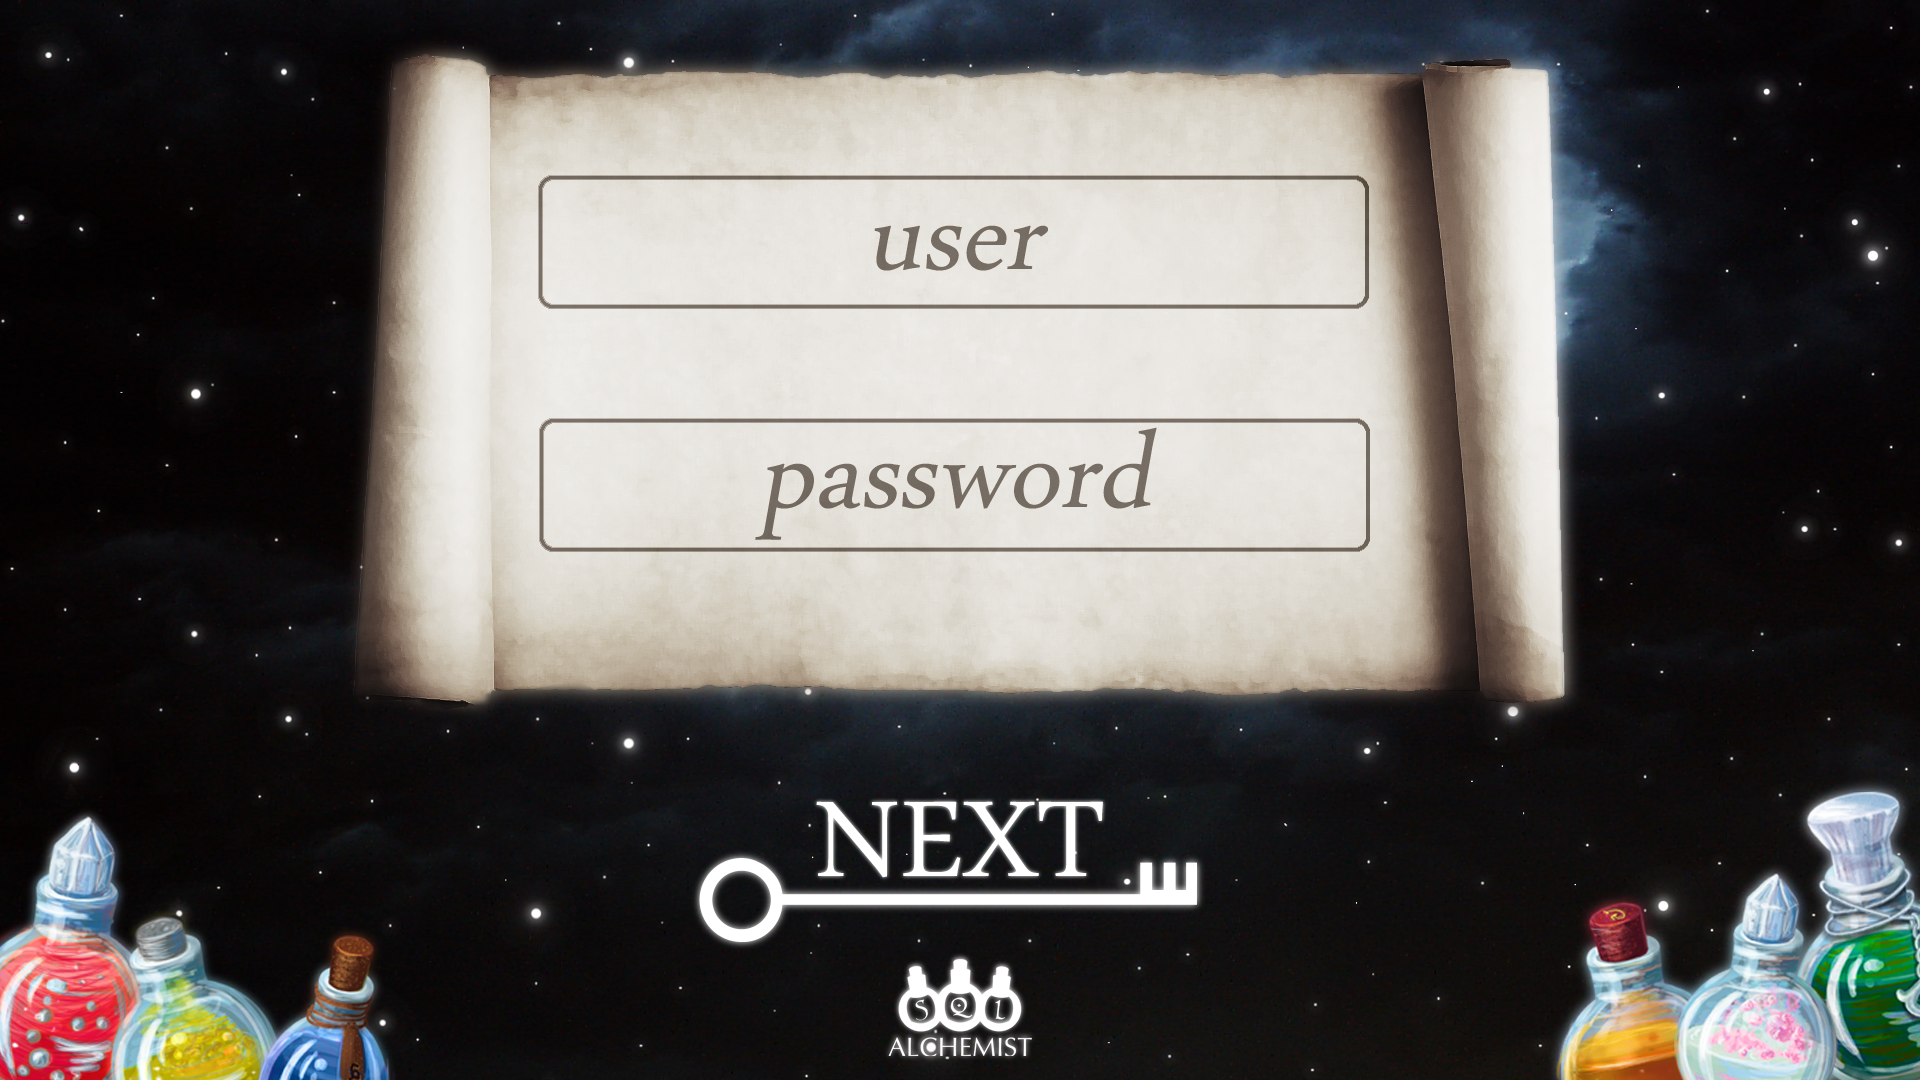
\includegraphics[width=0.7\textwidth]{figures/login_screen.png}
\caption{Login}
\label{gui}
\end{figure}
\end{ui}

\begin{ui}{30}{Minispiel-HUD}
Das Minispiel wird über die Maus gesteuert. Durch Klicks kann der Spielcharakter springen. Durch das Klicken der Potions im linken
unteren Rand des Screens können diese ebenfalls eingesetzt werden.
Durch das Klicken des „Beenden“-Buttons, dargstellt durch ein X, kann das Minispiel befrüht beendet werden.
\end{ui}

\begin{ui}{40}{SQL-Trainer-Screen}
Hier wird es dem User möglich sein, eine Aufgabe zu lösen. Dies geschieht über die Eingabe in ein Textfeld. 
Über einen Button kann das eingegebene Statement auf Korrektheit überprüft werden. Eventuelle Fehlerhinweise
werden ebenfalls in einem Textfeld visualisiert.
\end{ui}

\begin{ui}{20}{Menüführung}
\begin{figure}[ht]
\centering
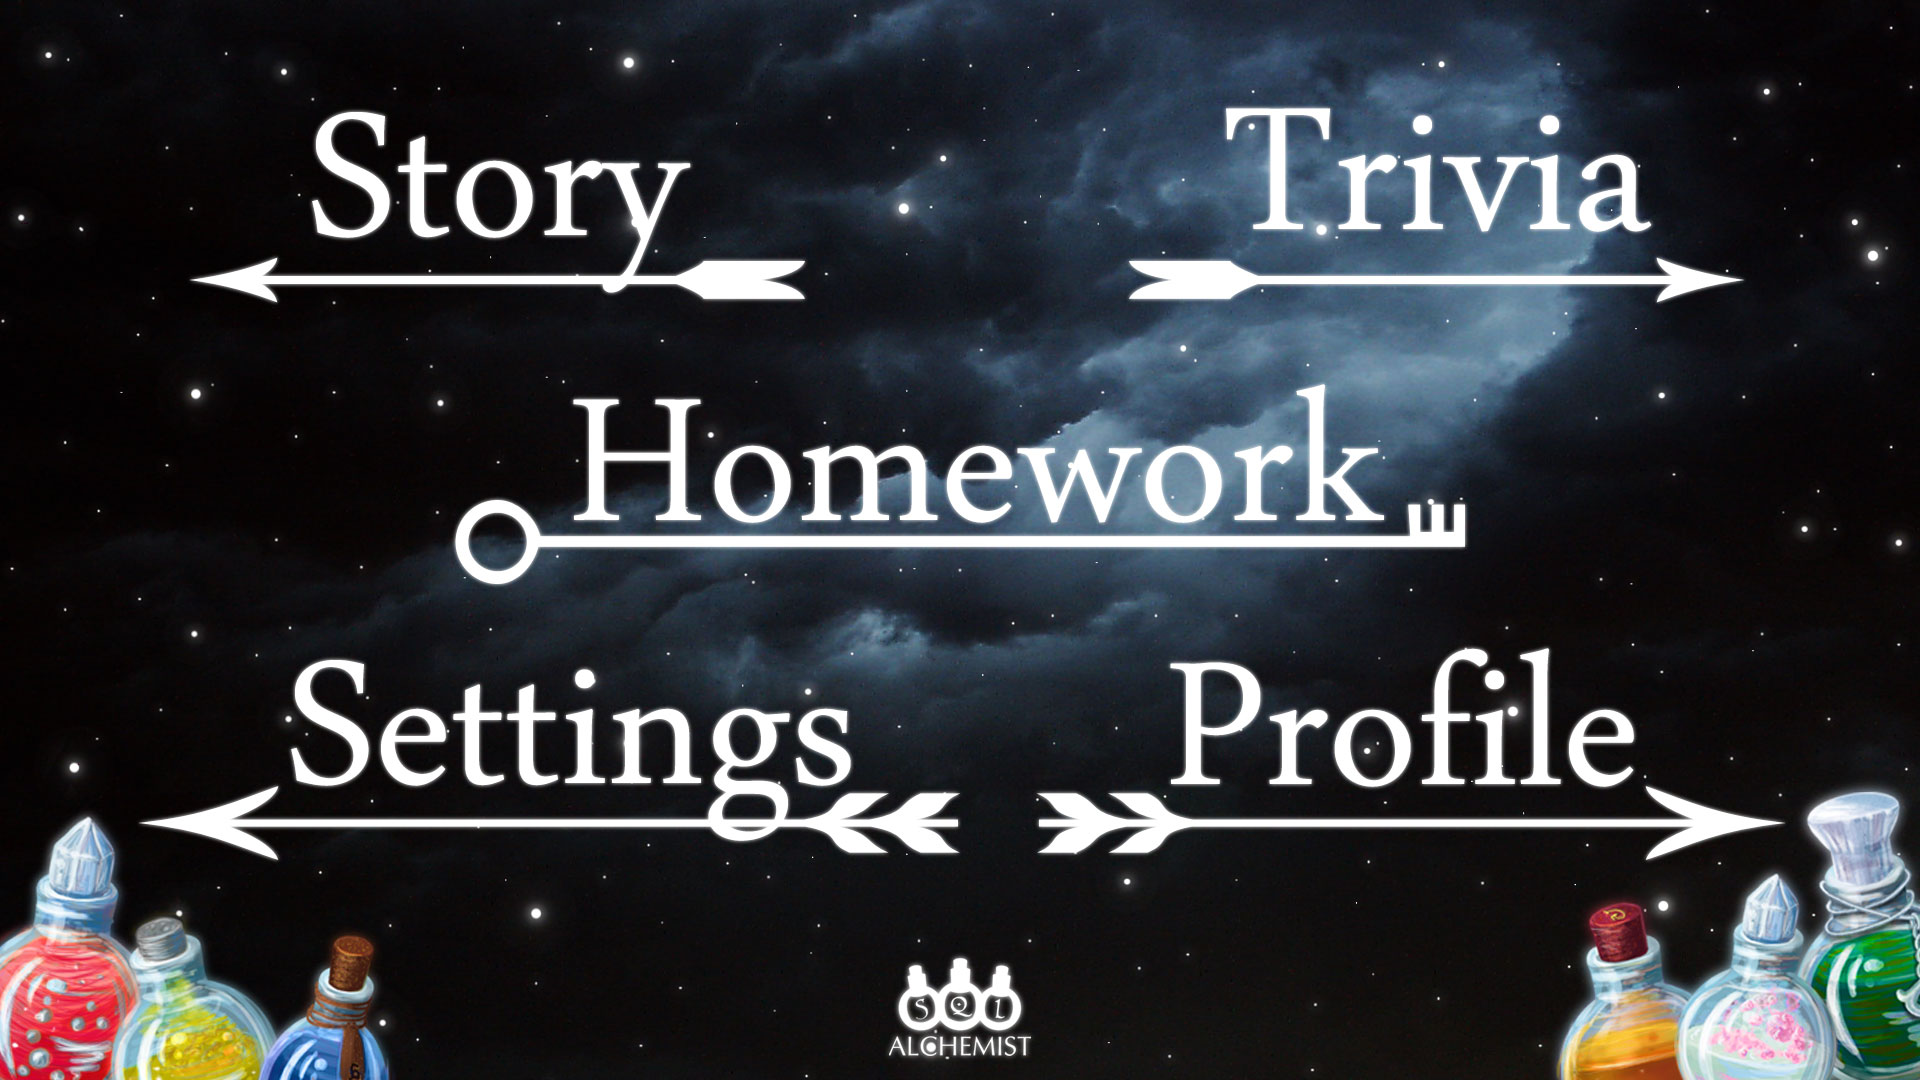
\includegraphics[width=0.7\textwidth]{figures/home_screen.png}
\caption{Men\"uf\"uhrung}
\label{gui}
\end{figure}
Das Hauptmenü ist dass zentrale Userinterface zur Kotrolle des Programmablaufes. 

Hier kann der User über Mauseingaben entweder weitere Teilmenüs 
aufrufen, wie den Trivia-, den Storymodus. Auch die Ranglisten k\"onnen in diesem Men\"u eingesehen werden.
Weiterhin bietet sich den Studenten unter den Usern die Möglichkeit, sich ihren Hausaufgaben zu widmen. Hierf\"ur ist ebenfalls eine eigener Men\"upunkt 
vorgesehen. Au{\ss}erdem gibt es die Möglichkeit sich in das Untermenü der Settings zu begeben, wo der User s\"amtliche Einstellungen ver\"andern kann.
\end{ui}


\begin{ui}{50}{Admin-Tool}
\begin{figure}[ht]
\centering
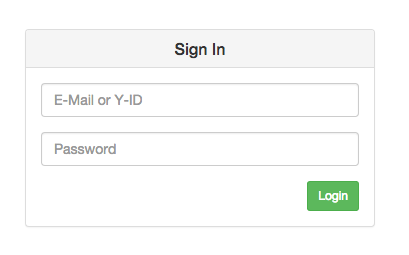
\includegraphics[width=0.7\textwidth]{figures/sign_in_admintool.png}
\caption{Login zum Admin-Tool}
\label{gui}
\end{figure}
Das Admin-Tool ist das zentrale Userinterface zur Kotrolle der User- und Aufgabenverwaltung. Hier kann sich der User einloggen um nachzuschauen ob er die 
Hausaufgaben bestanden hat oder nicht. Des Weiteren kann sich hier der Admin anmelden um Einstellungen zu ver\"andern oder Aufgabenpakete in die Datenbank 
einzupflegen. Jeder bef\"ordete User wird die M\"oglichkeit haben \"uber diesen Login selbst SQL-Aufgaben zu erstellen.   
\end{ui}




%!TEX root = ../Pflichtenheft.tex

% Kapitel 10
% Die Unterkapitel können auch in separaten Dateien stehen,
% die dann mit dem \include-Befehl eingebunden werden.
%-------------------------------------------------------------------------------

\chapter{Technische Produktumgebung}

\section{Software}

Front-End/ Minispiel:
\begin{itemize}
	\item beliebiges Betriebssystem
	\item ein g\"angiger Browser
	\item aktiviertes Javascript im Browser
\end{itemize}

Back-End/ Administration:
\begin{itemize}
	\item ein gängiger Browser
	\item Datenbank
	\item LDAP-Anbindung zur Studentenverifizierung
\end{itemize}


\section{Hardware}

Front-End:
\begin{itemize}
	\item Standard PC oder browserfähiges Gerät
\end{itemize}

Back-End:
\begin{itemize}
	\item Server
\end{itemize}


\section{Produktschnittstellen}

Die Teamprojekt-Software wird nativ in die Serverapplikation integriert.

Die Serveranwendung besitzt eine Kommunikations-Schnittstelle zum LDAP derTechnischen Universit\"at Braunschweig.

%!TEX root = ../Pflichtenheft.tex

\chapter{Glossar}

Belt: Die vom Spieler ausgew\"ahlten Potions, die er im Dungeon verwenden kann.

Character-Sheet: Eine \"Ubersicht \"uber die Attribute der Spielfigur.

Dungeon: Eine Aneinanderreihung von Leveln, die das Minispiel repr\"asentieren. 

Inventory: Im Inventory wird die Anzahl der aktuell vorhandenen Potions gespeichert.

Scrollcollection: Beschreibt den Fortschritt des Spielers indem es die bereits gesammelten Scrolls speichert. 

Herausforderung im Dungeon: Jede f\"unfte Map besitzt eine solche Herausforderung. Sie ist nur \"uberwindbar wenn mehrere Attribute der Spielfigur auf erh\"ohten Stand sind. Beispiele w\"aren eine extrem weite Schlucht oder einen besonders gro{\ss}en Gegner.

Playerstatistics: Attribute des Spielers, die Auswirkungen auf das Minispiel haben (Sprungh\"ohe, Geschwindigkeit, Leben und St\"arke).

Potions: Die im Spiel verwendete Bezeichnung f\"ur Tr\"anke, die dem Spieler tempor\"are Vorteile
verschaffen. Sie werden durch das richtige Bearbeiten von SQL-Anfragen erstellt werden k\"onnen. 

Scrolls: Einmalig im Spiel im einzusammelnde Objekte. Besitzt man diese, ist man in der Lage durch das L\"osen von SQL-Statements Potion zu erstellen oder die Playerstatistics dauerhaft zu erh\"ohen. 

Scroll-/Coin Limit: Gesetztes Limit, das die Anzahl an einsammelbaren Coins beziehungsweise Scrolls pro Tag bestimmt.

Scenetexts: Texte, die die Story und das Tutorial erz\"ahlen.


%------Ende des Dokumentes------------------------------------------------------
\end{document}
